\documentclass[article,shortnames]{jss}
%%%%%%%%%%%%%%%%%%%%%%%%%%%%%%
%% declarations for jss.cls %%%%%%%%%%%%%%%%%%%%%%%%%%%%%%%%%%%%%%%%%%
%%%%%%%%%%%%%%%%%%%%%%%%%%%%%%

\usepackage{amssymb}

%% almost as usual
\author{Stefan R\"odiger$^{\ddag,\S}$\\L.U.A.S. \& Charit\'e
	\And ~	% HACK to avoid over-printing of names
	\And Thomas Friedrichsmeier$^{\ddag,\S}$\\Ruhr-University Bochum
	\And ~
	\And Prasenjit Kapat\\The Ohio State University
	\And ~
	\And Meik Michalke\\Plus Affiliation
}
\title{RKWard - A Comprehensive Graphical User Interface and Integrated Development Environment for Statistical Analysis with \proglang{R}}

%% for pretty printing and a nice hypersummary also set:
\Plainauthor{Stefan R\"odiger, Thomas Friedrichsmeier, Prasenjit Kapat, Meik Michalke} %% comma-separated
\Plaintitle{RKWard - A Comprehensive Graphical User Interface and Integrated Development Environment for Statistical Analysis with {R}} %% without formatting
\Shorttitle{RKWard a GUI for \proglang{R}} %% a short title (if necessary)

%% an abstract and keywords
\Abstract{
  \proglang{R} is a free open-source implementation of the \proglang{S} statistical computing
language and programming environment. The current status of \proglang{R} is a
command line driven interface with no advanced cross-platform Graphical User
Interface (GUI) but it includes tools for building such. Over the past
years proprietary and non-proprietary GUI solutions, based on internal
or external tool kits, with different scopes and technological concepts
have emerged. For example, \proglang{Rgui.exe} and \proglang{Rgui.app} have 
become the de facto GUI on the Windows and MacOS X platforms, respectively, for most users. 
In this paper we discuss RKWard which aims to be both a
comprehensive cross-platform GUI and an Integrated Development Environment
(IDE) for \proglang{R}. RKWard is based on the \proglang{KDE} software libraries. Statistical
procedures and plots are implemented using an extendable plugin
architecture based on \proglang{ECMAScript} (\proglang{JavaScript}), \proglang{R}, and \proglang{XML}. RKWard
provides an excellent tool to manage different types of data objects;
even allowing for seamless editing of certain types. The objective of
RKWard is to provide a portable and extensible \proglang{R} interface for both
basic and advanced statistical and graphical analysis while not
compromising on flexibility and modularity of the \proglang{R} programming
environment itself.

%%Hi Thomas, this is my suggestion for the authorship, keep in mind you are the boss
\line(1,0){40}
\item$^{\ddag}$Equal contribution, $^{\S}$Corresponding authors
%%
}
\Keywords{GUI, IDE, \proglang{R}, plugin, cross-platform}

\Plainkeywords{keywords, comma-separated, not capitalized, Java} %% without formatting
%% at \leftarrowst one keyword must be supplied

%% publication information
%% NOTE: Typically, this can be left commented and will be filled out by the technical editor
%% \Volume{13}
%% \Issue{9}
%% \Month{September}
%% \Year{2004}
%% \Submitdate{2004-09-29}
%% \Acceptdate{2004-09-29}

%% The address of (at least) one author should be given
%% in the following format:
\Address{
  Stefan R\"odiger\\
  Lausitz University of Applied Sciences (L.U.A.S)\\
  Department of Bio-, Chemistry and Process Engineering\\
  AND\\
  Center for Cardiovascular Research (CCR)\\
  Charit\'e, Germany\\
  E-mail: \email{stefan\_roediger@gmx.de}\\
  E-mail: \email{rkward-devel@lists.sourceforge.net}\\
}

%% NOTE: It appears only the last entered address is actually used. So I guess we should only give Stefan's (the corresponding author).
% \Address{
%  Prasenjit Kapat\\
%  Affiliation\\
%  Department\\
%  E-mail: \email{noname@here.org}
% }
% \Address{
%  Meik Michalke\\
%  Affiliation\\
%  Department\\
% }


%% for those who use Sweave please include the following line (with % symbols):
%% need no \usepackage{Sweave.sty}

%% end of declarations %%%%%%%%%%%%%%%%%%%%%%%%%%%%%%%%%%%%%%%%%%%%%%%

\begin{document}

%% include your article here, just as usual
%% Note that you should use the \pkg{}, \proglang{} and \code{} commands.

% !TEX root = RKWard_paper.tex
\section{Background and motivation}
\label{background}
In mid 1993 Ihaka and Gentleman published initial efforts on the computing
language and programming environment \proglang{R} on the \emph{s-news} mailing list. Ambitions for
this project were to develop an \proglang{S}-like language without inheriting memory
and performance issues. The source code of \proglang{R} was finally released in 1995, and 
since 1997 development has evolved under the umbrella of the \proglang{R} 
Development Core Team \citep{RDCT2001, RDCT2010, Ihaka_Gentlemen_1993}.
\proglang{R} does not include an advanced cross-platform graphical user interface (GUI) as known from other
statistical software packages. However, \proglang{R} includes tools for building GUIs
mainly based on \proglang{Tcl/Tk} \citep{Dalgaard2001, Dalgaard2002}. Meanwhile a
plethora of \proglang{R} GUIs have emerged \citep[see][for a comprehensive list]{RGUI}. In 2005 John Fox released version 1.0 of \proglang{R} Commander \citep[package \pkg{Rcmdr}]{Fox2005}, which
can be considered a milestone in \proglang{R} GUI development; it was the first GUI
implementation that was able to make statistical tests,
plots and data manipulation easily accessible for \proglang{R} novices.
John Fox stated that \pkg{Rcmdr}'s target was to provide
functionality for basic-statistical courses, though the features have increased over
time beyond this \citep{Fox2005, Fox2007}. In November 2002 Thomas Friedrichsmeier
started the \pkg{RKWard} open-source software project with the goal to create a GUI for
\proglang{R} based on \pkg{KDE}\footnote{
  \pkg{KDE} is a desktop environment and software collection based on \pkg{Qt} (http://www.kde.org/).
  In the context of this paper, the term \pkg{KDE} is primarily used to refer to the programming library and
  runtime environment of \pkg{KDE}, rather than the complete software collection. For an introduction to
  \pkg{KDE} as a programming library, see \cite{Faure2000}.
} and \pkg{Qt}\footnote{
  \pkg{Qt} is a \proglang{C++}-based cross-platform programming library with a focus on GUI development
  \citep{BlanchetteSummerfield2008}. Online documentation is available at http://qt.nokia.com/.
} technologies.

The scope of \pkg{RKWard} is deliberately broad, targeting both \proglang{R} novices and experts.
For the first group, the aim is to allow any person with knowledge on
statistical procedures to start using \pkg{RKWard} for their everyday work 
without having to learn anything about the \proglang{R} programming language,
at least initially. At the same time, \pkg{RKWard} tries to support users who want to learn and
exploit the full flexibility of the \proglang{R} language for automating or customizing
an analysis. At the other end of the learning curve, \pkg{RKWard} provides advanced integrated development environment (IDE)
features to \proglang{R} experts to assist in writing \proglang{R} scripts. Yet, the idea
is that \proglang{R} experts too will benefit from the availability of task-oriented GUI
dialogs, such as when exploring an unfamiliar type of analysis
or by allowing to implement routinely performed tasks as a GUI element. In
addition, many features like the integrated data editor and the plot preview 
will be useful to \proglang{R} novices and \proglang{R} experts alike in their everyday work
(see Section~\ref{sec:user_interface}).

\pkg{RKWard} provides a high level of transparency about the steps that are needed to
perform any supported task in \proglang{R}, in order to make it easy for the user to see
complete codes for all GUI actions\footnote{
  This distinguishes \pkg{RKWard} from \proglang{R} GUIs such as \pkg{Red-R} (http://www.red-r.org/), which 
  specifically aims to hide the complexities of the \proglang{R} programming language, following the concept of visual data-flow 
  programming \citep{Sutherland1966}. In contrast, \pkg{RKWard} limits itself to generate \proglang{R} code from GUI settings.
}. In doing so, \pkg{RKWard} deliberately generates
comparatively verbose code. It avoids wrapping complex sequences of data
manipulation or analysis into custom high-level \proglang{R} functions. The task of
providing high-level functions is logically independent of the development of the
GUI frontend, and should best be addressed in dedicated \proglang{R} packages, where necessary.
This approach allows to make better use of the modular design of \proglang{R}, avoids
locking-in users to a specific GUI application, and provides them with more options for
customizing the generated code patterns.

While \pkg{RKWard} tries to address users wishing to learn \proglang{R}, it is specifically not
designed as a teaching tool -- such as \pkg{Rcmdr} \citep{Fox2005} or \pkg{TeachingDemos} \citep{TeachingDemos2010} -- but as
a productive tool. Since its incarnation \pkg{RKWard} has gained acceptance for usage in peer-reviewed 
publications \citep{Zou2008, Zou2009, Rugg-Gunn2010, Yang2011, Roediger2011, Roediger_VS}.
Dialogs for statistical procedures in \pkg{RKWard} do not
necessarily show a one-to-one correspondence to the underlying steps in \proglang{R}, but are
rather oriented at statistical tasks. Furthermore, \pkg{RKWard} does not impose
artificial limitations on how users can work with the application. For example,
the user is not limited to using only one \code{data.frame} or one model at a
time.

\pkg{RKWard} is designed to allow users to create custom GUI dialogs as plugins, requiring relatively
little programming knowledge. In essence, \pkg{RKWard} plugins consist of an XML file describing
the dialog layout, and \proglang{ECMAScript} code which generates \proglang{R} code from the settings
made in the GUI. Most of the data handling functionality in \pkg{RKWard} is implemented as plugins
(see Section~\ref{sec:analyzing_data}), and many of these plugins have originated as user contributions.
Since version 0.5.5, \pkg{RKWard} also provides support for downloading user contributed ``plugin packs'',
which are not included in the official \pkg{RKWard} releases. Details on the definition of plugins,
and a commented example can be found in the technical supplement to this article.

\pkg{RKWard} is licensed under the terms of the GNU General Public License\footnote{http://www.gnu.org/licenses/gpl.html} Version 2
or higher. However, due to its dependencies, \pkg{RKWard} binaries are effectively
distributable only under the terms of Version 2 of the license. Parts of the documentation are available under the
GNU Free Documentation License\footnote{http://www.gnu.org/licenses/fdl.html}. While the project remains in constant development, a growing
number of users employs \pkg{RKWard} in productive scenarios. The source code,
selected binaries and documentation is hosted at SourceForge
(\url{http://rkward.sourceforge.net/}). Selected key milestones of the development of \pkg{RKWard} are
visualized in Figure~\ref{fig:timeline}.

In this paper we will give an overview over the installation process (Section~\ref{sec:installing_starting_RKWard}), the main GUI elements and
features of \pkg{RKWard} (Section~\ref{sec:user_interface}), and closing by a short example 
of a simple \pkg{RKWard} session (Section~\ref{sec:using_RKWard}). For readers interested in the technical
design, and reasons for certain design decisions, a technical supplement to this article
is available.

\begin{figure}[t!]
 \centering
 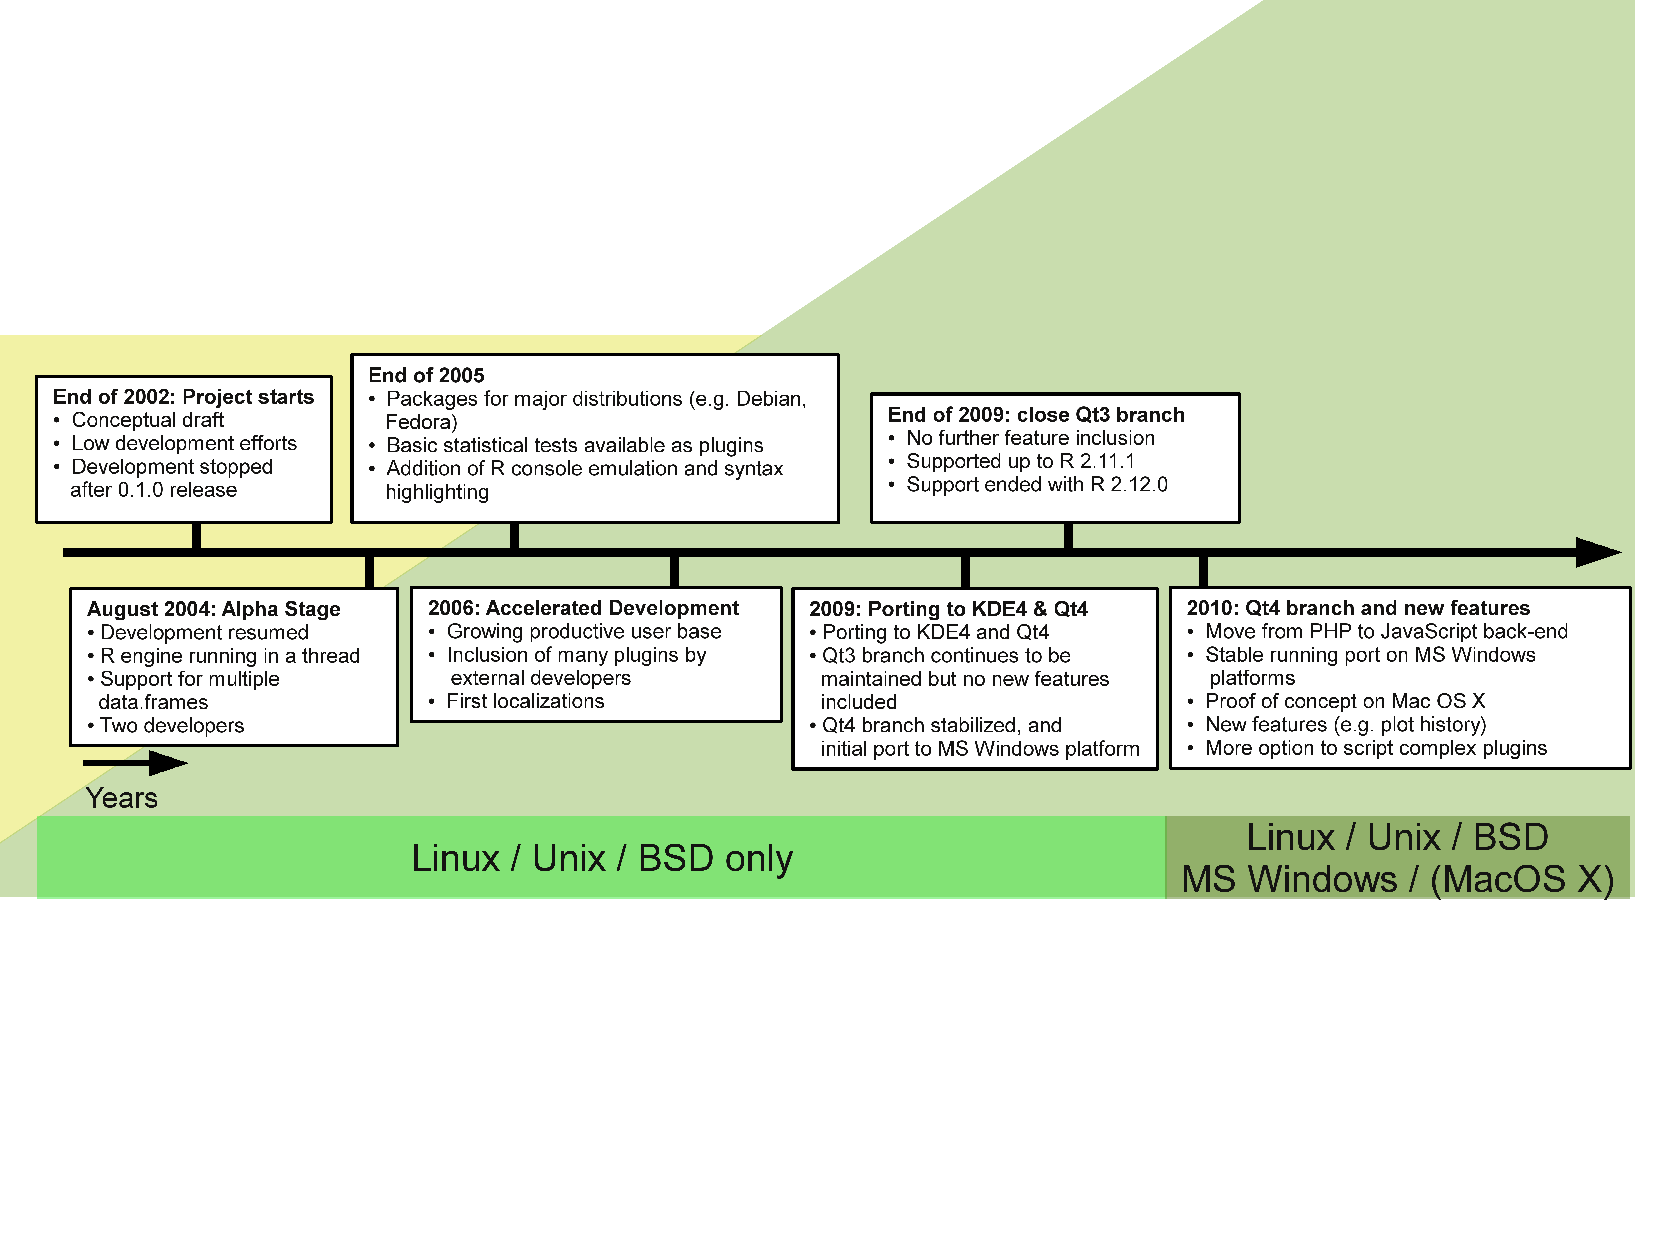
\includegraphics[clip=true,trim=0cm 5.7cm 0cm 5.7cm,width=15.4cm]{./figures/timeline.pdf}
 \caption{Timeline of important development milestones and changes in \pkg{RKWard}.
          Time is presented on an arbitrary scale. Here \pkg{Qt}3 and \pkg{Qt}4 refers to the 3.x and
          4.x versions of the \pkg{Qt} libraries, respectively and \pkg{KDE}4 refers to the
          4.x version of the \pkg{KDE} libraries.}
 \label{fig:timeline}
\end{figure}

\section{Installation and platform availability}
\label{sec:installing_starting_RKWard}
Contrary to some other \proglang{R} GUIs, such as \pkg{Rcmdr}, \pkg{RKWard} cannot be installed and started as a
regular \proglang{R} add-on package. Rather, it is started as a stand-alone application which embeds the
\proglang{R} engine, and needs to be installed in a platform dependent way, as detailed, below\footnote{
  See http://p.sf.net/rkward/download for an overview and platform specific download links.
}. Besides the
\pkg{KDE} runtime environment and \proglang{R}, \pkg{RKWard} utilizes a growing number of \pkg{R} add-on packages.
However, these do not have to be installed before hand. Rather \pkg{RKWard} will prompt the user to install
missing packages, interactively, on an as-needed basis (see Section~\ref{sec:package_management}).

\subsection{Installation on the GNU/Linux platform}
Historically, \pkg{RKWard} originates on the GNU/Linux platform, and binary packages are available for many major
distributions, including Debian, Ubuntu, OpenSuse, Gentoo, Fedora, and also FreeBSD. On systems which
provide up-to-date packages of \proglang{R} and \pkg{KDE}, compilation from source is generally unproblematic\footnote{
  See http://p.sf.net/rkward/compilling for details.
}. The exact size of the installation is system dependent. On Debian x86, the package is currently around 1.5 MB (Megabyte) compressed,
and 5.5MB uncompressed. However, if the \pkg{KDE} runtime environment is not yet installed, an installation of \pkg{RKWard} may
need several hundred MB of disc space.

\subsection{Installation on Microsoft Windows}
\pkg{RKWard} can be used on Windows XP, Windows Server 2003, Vista, and Windows 7. Source installation on the
Microsoft Windows platform is comparatively difficult, since various tools need to be installed\footnote{
  See http://sourceforge.net/apps/mediawiki/rkward/index.php?title=RKWard_on_Windows/Packaging for details.
}, however, 32bit binaries are also provided by the project. The user has a choice between an small installer (1.7 MB),
which can be used to install \pkg{RKWard} to pre-existing installations of \proglang{R} and \pkg{KDE}, and a installation
bundle, which includes \pkg{RKWard}, \proglang{R}, and \pkg{KDE}. This bundle can be unpacked to any user-writable folder,
and can be run without any further steps of installation. Using this method of installation,
\pkg{RKWard} can also be installed to a removable storage medium, and moved between different systems (configuration
settings are stored in the user's home directory, and will not be shared across systems, unless the user takes further steps).
The size of the current installation bundle is 132 MB compressed, and around 670 MB installed.

\subsection{Installation on Mac OS X}
At the time of this writing, the developers lack the resources to support a Mac OS X port, and especially
to provide binaries for Mac OS X. \pkg{RKWard} has been successfully compiled and installed on the Mac, and
appeared to be mostly functional, but there have also been unresolved reports of failure to compile or to start
\pkg{RKWard} on Mac OS X. Since \pkg{KDE} project does not currently offer binaries for Mac OS X, installation
of \pkg{RKWard} also requires compilation of the \pkg{KDE} runtime environment, and its dependencies from source,
which takes many hours to complete on current systems. Further, \pkg{RKWard}'s grapics device window related features
(see Section~\ref{sec:plot_previews}) are only available when compiling and using \pkg{KDE} and \pkg{RKWard} in
\pkg{X11} mode. In conclusion, \pkg{RKWard} on Mac OS X cannot currently be considered ready for regular users.

\subsection[Starting RKWard]{Starting \pkg{RKWard}}
\pkg{RKWard} cannot be loaded from within an \proglang{R}
session, but rather it is started as a stand-alone application with an
embedded \proglang{R} engine. To facilitate the first
steps for new users, a dialog offers the choice to load an existing
workspace, to start with an empty workspace, or to create a new
\code{data.frame} and open that for editing. Also, an overview help page is
shown in the document area of the main window. Both start-up features
can be turned off.

\section{Main elements of the user interface}
\label{sec:user_interface}
This section gives an overview of the main user interface elements and features of RKWard.
For a use case oriented example of an RKWard session, see Section~\ref{sec:using_RKWard}.

The default layout\footnote{
 Many aspects of the RKWard GUI can be customized by the user. For simplicity we will
 describe the default appearance of RKWard, only.
} of the main application window is divided into five
parts, as depicted in Figure~\ref{fig:main_window}. The top of the window is occupied by menu bar and toolbar 
(Figure~\ref{fig:main_window}A). The content of both bars is partially context
sensitive, e.\,g., the ``Edit'' menu will offer
one set of actions when the current document window is a data editor,
and another set of actions for a \proglang{R} script
editor window. To ease orientation, all top level menus remain
persistent, even if no actions are available for that menu in the
current context. The menu bar of the main window is also the central
access point to most data import, manipulation, analysis, and
visualization features (see Section~\ref{sec:analyzing_data}) for which RKWard provides a GUI
interface.

\begin{figure}[htp]
 \centering
 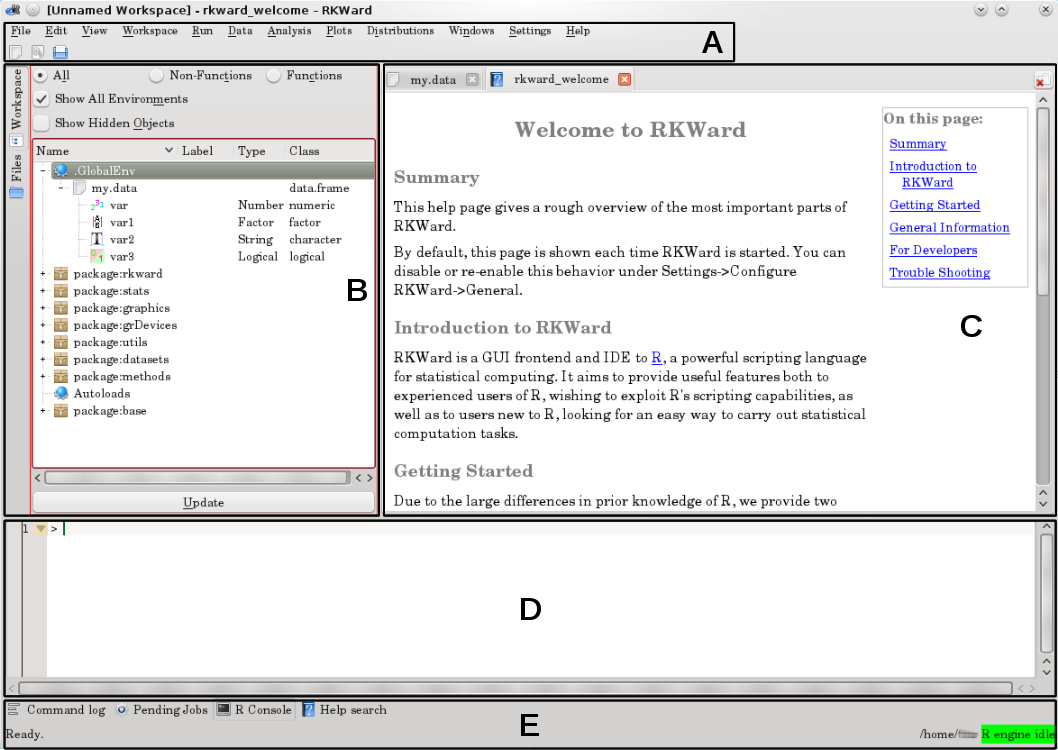
\includegraphics[width=15.450cm]{../figures/main_window.png}
 \caption{Default RKWard main window after start up. 
A) Menubar and toolbar, B) tool panel showing workspace browser, C) main view area, showing
a help page D) tool panel showing embedded \proglang{R} console E) tool buttons, and status bar.
Panels B) and D) can be resized or collapsed. Note the red square (B) indicates the active interface element.}
 \label{fig:main_window}
\end{figure}

A status bar is shown at the bottom of the window (Figure~\ref{fig:main_window}E). It displays (from
right to left) the status of the \proglang{R} engine (busy or idle), the
current working directory, and a multi purpose region for additional
information on some menu items and other GUI elements, visible when
hovering the mouse pointer over them.

The central area is divided into a document view area
(Figure~\ref{fig:main_window}C) and two panel subwindows
(Figure~\ref{fig:main_window}B and D). The panels can be resized or moved to
another edge of the central area independently. All panels can be
toggled by mouse or keyboard shortcuts. When a panel is closed, the
document view area (see below) is automatically re-sized to take up the
free space.

The left panel (Figure~\ref{fig:main_window}B) contains a file browser (see Section~\ref{sec:further_tool_windows}) and a
workspace browser (see Section~\ref{sec:workspace_browser_object_viewer}) by default. The
bottom panel (Figure~\ref{fig:main_window}D) contains the tool windows, namely, Command
log (Section~\ref{sec:further_tool_windows}), Pending Jobs (Section~\ref{sec:further_tool_windows}), \proglang{R} Console
(Section~\ref{sec:using_R_console}), and Help Search (Section~\ref{sec:help_system}).

The remainder of the central area (Figure~\ref{fig:main_window}C) is a single row tabbed document
interface (TDI) for different documents. Early uses of TDIs date back to 1988 and are
widely applied nowadays \citep{Hopkins2005, MDN2010,
KimLutteroth2010}. Currently, the supported types of
documents are object summaries (Section~\ref{sec:workspace_browser_object_viewer}), 
script editors (Section~\ref{sec:code_editor}), spreadsheet-like data editors 
(Section~\ref{sec:spreadsheet}), results output (Section~\ref{sec:results_output}), 
help pages (Section~\ref{sec:help_system}), and also
\proglang{R} on-screen graphics devices (Section~\ref{sec:technical_graphics}). 
The order of tabs can be conveniently re-arranged
using drag \& drop.

All document windows and tool views can be detached and re-attached from the main
window as independent windows, managed by the window manager. This feature allows to 
conveniently work with multiple documents
at the same time, e.\,g., scripts or data editors. On{}-screen
graphics device windows are created detached by default, but can 
be attached to the document view area of the main window.

Windows can be shown (or toggled) using a mouse device with point \&
click, as well as using a series of keyboard shortcuts (defined by
default) for switching between the different tool and document windows.
Key bindings can be configured from the GUI via ``Settings$\rightarrow$Configure Shortcuts''. 
However, for technical reasons only the shortcuts of currently active components 
will be listed. Thus, for example, to
configure data editor shortcuts, one has to open a data editor first and
then to select ``Settings$\rightarrow$Configure Shortcuts''. Since RKWard relies on the 
\proglang{KDE} SC editor component,
shortcuts for the script editor (Section~\ref{sec:code_editor}) are managed separately via 
``Settings$\rightarrow$Configure Editor$\rightarrow$Shortcuts''. On most systems, it is also
possible to configure shortcuts by right-clicking on the respective
menu item.

The choice of available actions on the tool bar can be
configured via ``Settings$\rightarrow$Configure Toolbars''. Further, it is possible to add and remove sets
of data manipulation and analysis features from the GUI, using
``Settings$\rightarrow$Configure RKWard$\rightarrow$Plugins''.

\subsection{Workspace browser and object viewer}
\label{sec:workspace_browser_object_viewer}

The workspace browser (Figure~\ref{fig:main_window}B) allows to view
and manipulate \proglang{R} objects, similar
to a regular file-system browser. This includes both, user objects
(data, functions, environments) in \code{.GlobalEnv} and non-user objects in other environments in the
\proglang{R} search path (typically,
\proglang{R} package environments). Objects are shown
in a hierarchical tree structure. For instance, an object of class
\code{list} can be expanded to show all contained objects 
by clicking on the $+$ symbol left of the object name.
The basic type of each object is indicated by specific icons. Further
information on each object can be seen by hovering the mouse
pointer over the respective icon. A tooltip window will appear,
including information such as dimensionality or function arguments,
depending on the type of object. Further, objects inside \code{.GlobalEnv} can be
removed, renamed, and edited from the context menu.

Several actions are available from a context menu (after right-clicking
on the object names), depending on the type of object. These allow to search the
\proglang{R} help for information on that object, to
open a window with detailed information on the object, to delete, rename or copy the object to a new symbol name, or to
copy it to \code{.GlobalEnv}. Further, the context menu allows to open
supported types of objects for editing (see Section~\ref{sec:spreadsheet}; currently, only
\code{data.frame}s can be edited, and only while they exist in \code{.GlobalEnv}). 
Selecting ``View'' from the 
context menu opens a new window in the
document area, containing basic information on the object as well as 
tabs which show the output of
\code{print()} and \code{summary()} calls.

Literally hundreds or even thousands of objects are present in a typical
\proglang{R} session. This can be overwhelming at
first, therefore, the workspace browser has options to show only a certain
subset of objects, e.\,g., only functions or only data objects, including
or excluding hidden objects (object names starting with a 
``.''), or showing only the contents of \code{.GlobalEnv} as
opposed to all environments in the search path.

An object list similar to the workspace browser (but showing only 
\code{.GlobalEnv} by default) is also used in several places for the
selection of objects to work with, e.\,g., in an analysis plugin (see Section~\ref{sec:analyzing_data}).


\subsection{Code editor}
\label{sec:code_editor}

RKWard comes with an advanced
\proglang{R} script editor, based on the
\proglang{KDE} advanced text editor component (Kate; \url{http://kate-editor.org/}). Features of this
editor include syntax highlighting (both on screen and in printouts; for
\proglang{R} and many other script types), code
folding, block-wise indentation adjustments or commenting, automatic
brackets, search and replace with plain text or regular expressions,
and many more. The editor automatically saves snapshots of the
currently edited files at configurable intervals.

For interaction with \proglang{R}, the editor has
predefined shortcuts (and toolbar icons) for submitting the current line, the current 
selection, predefined blocks, or the entire document to the
\proglang{R} engine for evaluation. It also 
offers object name completion and function argument hinting 
(Figure~\ref{fig:code_hinting}A and B) based on the objects present in
the \proglang{R} workspace\footnote{The object name
completion and function argument hinting features in RKWard predate the
inclusion of similar features into the core
\proglang{R} distribution. For this reason, they are
technically based on different mechanisms.}. A further feature specific
to the \proglang{R} language is the
``Paste Special'' action, which allows to
paste the clipboard content (e.\,g., from a separate spreadsheet
application) as a single string, vector, or matrix, suitable
for inclusion in an \proglang{R} script, optionally
transforming it in advance (Figure~\ref{fig:special_paste}).

\begin{figure}[htp]
 \centering
 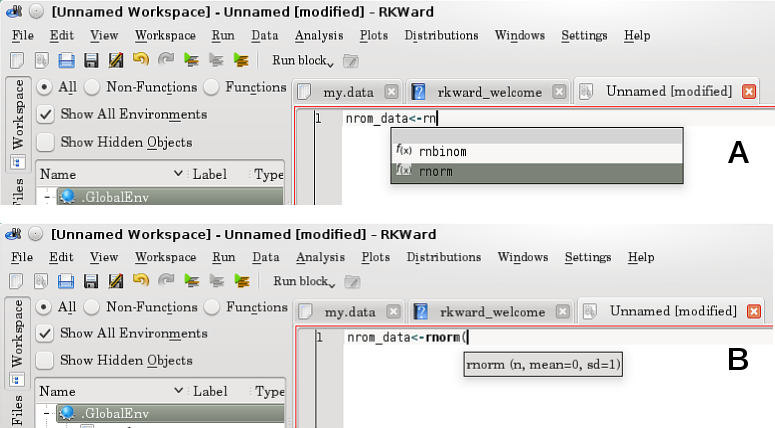
\includegraphics[width=15.5cm]{../figures/code_hinting.png}
 \caption{Code hinting features of the script editor. The script editor is able to hint A) \proglang{R} object names
and B) function arguments. Random data (\code{rnorm()}, n = 50) were assigned to a variable and later used in Figure~\ref{fig:plot_history}.}
 \label{fig:code_hinting}
\end{figure}

\begin{figure}[htp]
 \centering
 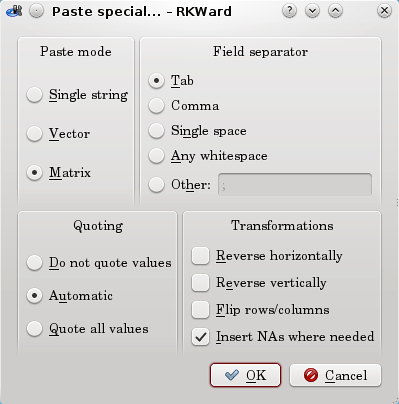
\includegraphics[width=8.042cm,height=8.143cm]{../figures/special_paste.png}
 \caption{Special paste dialog. This tool allows to paste data (e.\,g., tabular, text) from the clipboard, directly to an 
 \proglang{R} script and therefore accelerates the work process with data from different sources 
 like spread-sheet applications.
}
 \label{fig:special_paste}
\end{figure}

Script editor windows can be created by opening an existing
\proglang{R} script file from the file browser, the
``File'' menu, or by creating a new empty script. It can
also be invoked from \proglang{R}, e.\,g., using the
\code{file.edit()}, \code{file.show()}, or \code{fix()}
commands.

\subsection{Using the R console}
\label{sec:using_R_console}
For users with knowledge of \proglang{R}, RKWard provides direct access to the
embedded \proglang{R} engine in the
\proglang{R} console tool window. It is important to understand that technically this is an
emulation of \proglang{R} running in a console
session, not a real \proglang{R} session. This leads to a few subtle
differences, e.\,g., with respect to the command history feature in
\proglang{R}.

However, for most purposes RKWard's \proglang{R} console can be used exactly
like \proglang{R} running in a terminal. Adding to that, it provides many of the
features which are also available in the code editor (see Section~\ref{sec:code_editor}).
Most prominently, it supports syntax highlighting, code
folding, function argument hinting, object name completion, and pasting
vector or matrix data directly from the clipboard.

By default, any code that is submitted to the
\proglang{R} engine from the code editor or from help
pages, is sent through the \proglang{R} console.
However, it can be configured to the submitted in the background,
instead.
For further technical details, see Section~\ref{sec:technical}.

\subsection{Spreadsheet-like data editor}
\label{sec:spreadsheet}

Historically, one of the earliest
features of RKWard is a built-in spreadsheet-like data editor.
Currently, editing \proglang{R} objects of type
\code{data.frame} is possible. In contrast to the \code{data.frame} editing shipped
with the \proglang{R} core distribution, this editor
gives the illusion of ``in-place'' editing of data. New \code{data.frame}s can
be created and opened from the GUI, and existing objects can be opened
for editing from the workspace browser. For opening objects from
\proglang{R} code, the function \code{rk.edit()} can be used.
Figure~\ref{fig:data_editors} shows multiple \code{data.frame}s open for editing.

\begin{figure}[htp]
 \centering
 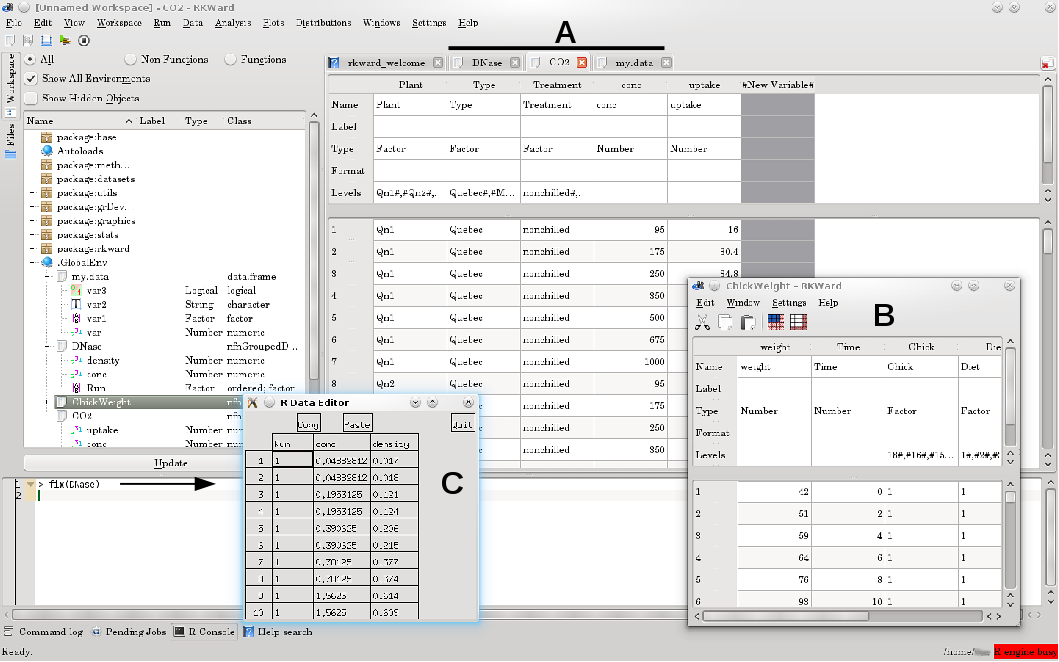
\includegraphics[width=15.5cm]{../figures/data_editors.png}
 \caption{RKWard with several \code{data.frame}s in use at the same time. A) 
  One \code{data.frame} is opened for editing in the main window. Two further \code{data.frame}s
  are opened in the background in tabs. 
  B) Another \code{data.frame} is opened as detached window. 
  C) \proglang{R}'s standard data editing features (e.\,g., \code{fix()}, \code{edit()}) 
  are also usable within an RKWard session. In this example \code{fix(DNase)} 
  was invoked from the console (arrow).}
 \label{fig:data_editors}
\end{figure}

Meta-data on each column of a \code{data.frame} (i.\,e., name of the column, data
type, and potentially data labels) is shown in the upper portion of
the data editor, and can be manipulated there, while the data itself is
shown in the lower portion. The upper portion can be hidden using a
slider, to save space for the display and editing of actual data.
Similarly, an editable column showing the row names of the \code{data.frame}
can be shown or hidden separately from the data.

For columns of type \code{factor}, factor levels can be edited by double-clicking on the
``Levels'' row of the meta information. Levels can also be assigned to other types of
variables, but only for consecutive integer values. These levels will
be displayed instead of the underlying value, if applicable. Each
column can also be assigned an arbitrary descriptive
``Label'', which is stored in
\proglang{R} as an attribute of the column.

Contrary to many other editors, the data editor in RKWard does not
automatically convert data types of columns. For instance, if a
non-numeric string is entered into a cell of a numeric column, the data
type of the column remains numeric, and the entered value is
highlighted in red. Internally, the invalid cell is set to \code{NA}.
The entered value is stored separately, in an attribute of the column.
The rationale for this approach is that it offers protection against
accidental, and probably undetected, conversion of data types. The
user can manually convert the storage mode of a column by simply
selecting a different data type in the ``Type'' row of the meta information.

The data editor supports insertion and deletion of rows or columns at 
arbitrary positions. Rows (columns) can also be added at the bottom 
(right) by simply entering data into the trailing row (column) shown in
gray. Copy \& paste is supported, where the area affected by paste
operations can optionally be constrained to the selected region, or to
the dimensions of the table. The data editor can also be set to read-only
mode to examine data objects.

In the context of data editing, it is noteworthy that
RKWard supports working with multiple objects simultaneously, rather than
limiting actions to a single active \code{data.frame}, as with e.\,g., \pkg{Rcmdr} or
\pkg{DeduceR}. Given this non-modal interface design, multiple data editor
windows can be opened at once (Figure~\ref{fig:data_editors}).

\subsection{Handling, manipulating, and analyzing data}
\label{sec:analyzing_data}

Dealing with data -- i.\,e., importing, transforming, filtering, analyzing, and visualizing  --
is the core strength of \proglang{R}, and one central goal of
RKWard is to make the most of this functionality available to a broader
audience by providing it in the form of easy to use GUI dialogs. Since
the data handling functionality itself is provided by
\proglang{R} and its numerous add-on packages, this
can basically be accomplished by defining GUI dialogs, generating
\proglang{R} code according to the settings made in
the GUI, and having the generated code evaluated by the
\proglang{R} engine. 
This general pattern, implemented as plugins, is the
basic recipe for most of the functionality provided by RKWard
(see Section~\ref{sec:technical_plugins} for details). For
the purpose of this article we will look at the standard
elements of data handling functions by example of importing CSV
(comma-separated values) data\footnote {
  Note that on purpose, RKWard does not have its
  own file format for data import and export, but rather uses
  \proglang{R} workspaces as default data format. Additionally, it is possible
  to import data from several sources as described in this section. Of course, further formats can
  also be imported using copy \& paste (see Sections~\ref{sec:code_editor} and \ref{sec:spreadsheet}), or by
  manually entering appropriate \proglang{R} commands in
  the \proglang{R} console (Section~\ref{sec:using_R_console}).
}. Further examples are given in Section~\ref{sec:using_RKWard}.

At the time of this writing, RKWard provides support for importing SPSS, 
Stata, and ``delimited text'' data. Internally, RKWard
relies on standard \proglang{R} functions and the package \pkg{foreign}
\citep{Murdoch2002} for reading these data files. To import CSV (comma separated values)
data, select ``File$\rightarrow$Import format$\rightarrow$Import Text$\rightarrow$CSV''
data from the menu. This will open the dialog shown in
Figure~\ref{fig:CSV_import}. The central area of this dialog provides 
options to control the import. The 
``File name'' field is highlighted, to indicate that
it is required to specify a file before the dialog can proceed.
Further options are available from the tabbed pages of the central area.

\begin{figure}[htp]
 \centering
 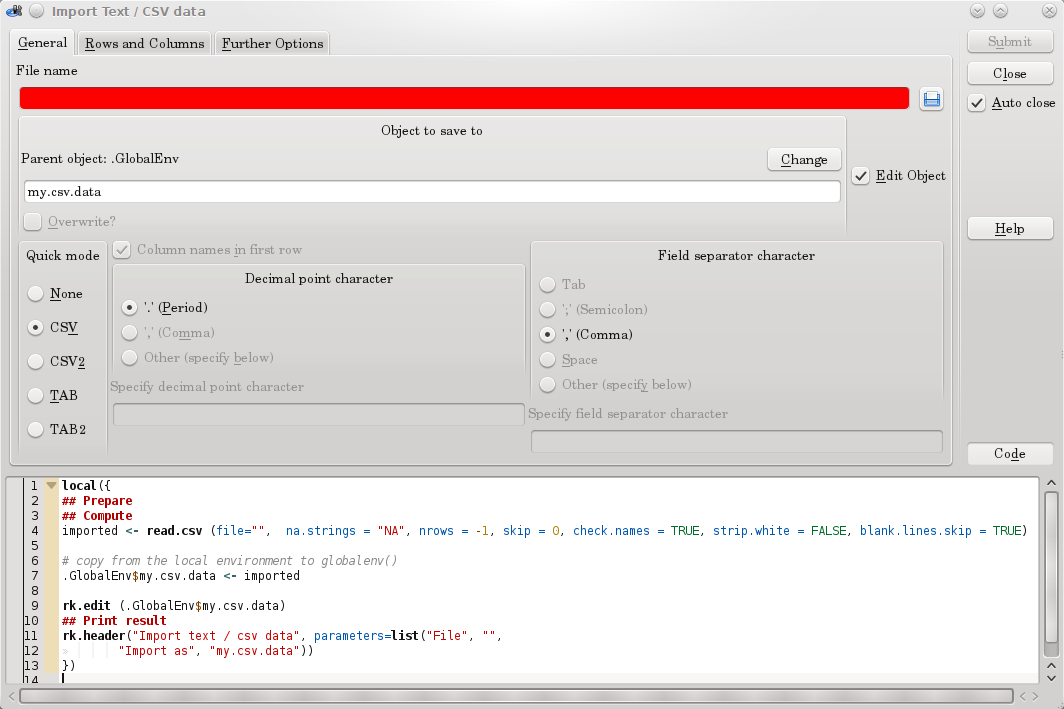
\includegraphics[width=15.5cm]{../figures/CSV_import.png}
 \caption{General data import dialog. Useful defaults for a variety of formats can
  be set using the ``Quick Mode'' selector on the left. Customizations can be done
  from the ``Rows and Columns'' and ''Further Options'' tabs, respectively. The 
  code in the bottom area can be copied and used for other purposes.}
 \label{fig:CSV_import}
\end{figure}

The right-side area is common to all data handling
dialogs. Here the ``Submit'' button is used
to start the import action. It is enabled once all required
settings have been made, i.\,e., in this case, once a file name has been
selected. The ``Close'' button will close the
dialog without taking any action.

The bottom area optionally shows the \proglang{R}
code corresponding to the current settings, and which will be run
upon pressing the ``Submit'' button (see Section~\ref{sec:importing_data} for generated \proglang{R} code). 
The code display is hidden by default and can be revealed using
the ``Code'' button. This 
generated code display is updated dynamically as the user changes settings, allowing
to see the effect of each change instantly.

Most data handling functions will produce some output, which is
sent to the output window. From there it is possible to repeat the
action by clicking on the ``Run again''-link
(see Section~\ref{sec:results_output}).

\subsection{Graphics window and plot previews}
\label{sec:plot_previews}

For plotting, RKWard relies on the graphics capabilities provided by
\proglang{R}. All \proglang{R}
devices, including on{}-screen devices, can be used in the regular way.
However, for the \code{X11()} and \code{windows()} devices, RKWard adds a menu
bar and a toolbar to the device windows (on the MS Windows platform,
replacing the default menu bar provided by the device). The menu
bar and toolbar give access to a number of different functions,
including GUI dialogs for exporting the current plot,
and adding a grid to an existing plot 
(works on only certain types of plots).

Further, a history mechanism is provided,
which stores created plots automatically and allows to navigate
back to earlier plots (Figure~\ref{fig:plot_history}). 
The history is available as a drop down list of the plot calls as well as using typical ``back''
and ``forward'' buttons on the toolbar.
The maximum number
of plots to record, as well as the maximum size of each individual plot,
is configurable from the settings menu. This plot history is shared
between the open on{}-screen device windows, yet they behave
independently. For example, if multiple devices display the same
plot, any modification (including deletion) of the plot on one device
renders its instances on other devices as ``new'' and hence can be added
back to the plot history. In addition, duplicating or closing a device
window records any unsaved plots to the history.

\begin{figure}[htp]
 \centering
 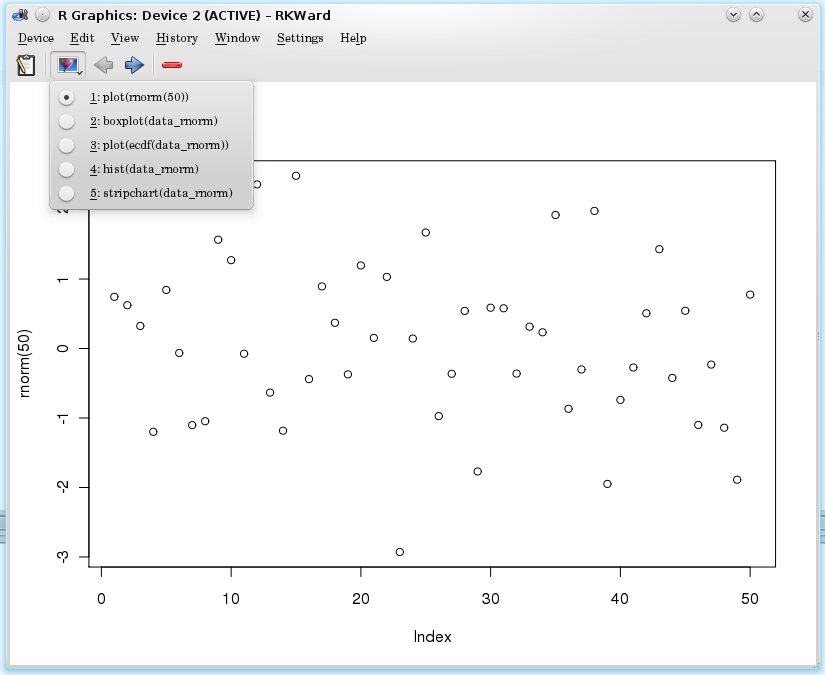
\includegraphics{../figures/plot_history_cropped.png}
 \caption{On{}-screen graphics device window in RKWard. The plot history is 
  available as a drop-down list, allowing to jump directly to a previous 
  plot. In this example, five different plots were performed on the same data 
  set of a random sample (\code{rnorm()}). The plot can be 
  exported via ``Device$\rightarrow$Export'' as described in Section~\ref{sec:create_plot}.
}
 \label{fig:plot_history}
\end{figure}

Further, RKWard provides access to different plotting functions using GUI dialogs,
available from the ``Plots'' menu. Wherever appropriate, RKWard supports a ``plot
preview'' feature. When the ``Preview'' box of
the respective dialog is checked (see Figure~\ref{fig:boxplot1}), a device window is opened, which
shows the plot as it would be created with the current settings. The
preview is updated automatically as the user makes changes, allowing to
see the effect of each setting instantly\footnote{The preview is
updated asynchronously to keep the GUI responsive; see Section~\ref{sec:technical_graphics}.}. For example, the CLT 
(central limit theorem) plugins
under the ``Distributions'' menu can be very helpful to dynamically ``show''
the convergence in distribution while teaching. For the sake of simplicity, such preview plots are not added to
the history.

\subsection{Results output}
\label{sec:results_output}

While all basic mechanisms of
capturing and documenting \proglang{R} output can also
be used, RKWard provides a dedicated output file and a output
window for documenting the results. All GUI-driven data handling
functions (see Section~\ref{sec:analyzing_data}) write their output to this file. 
The same applies to error messages, in case a plugin fails to perform its task.
The output is presented in a journal format\footnote{Note: The font size of the output can be adjusted
from the menu. 
Since it is based on \proglang{HTML}, it is also possible to view the source code 
(see below).}. All results are presented
sequentially with the last performed task at the bottom.
It is also possible to write to the output directly from \proglang{R}
scripts by using a number of dedicated \proglang{R}
functions included in the \code{rkward} package. For the GUI-driven data handling functions, the output is
standardized to include the name of the feature, the date and time of
its execution, and other basic parameters, wherever
applicable. Further, a clickable ``Run
Again'' link is rendered below the output of each data
handling feature, which allows to invoke the same feature again with
identical parameters\footnote{In case not all parameters could be
reused, since, may be, some of the objects in
question are no longer available, the user will be notified.} (see
Figure~\ref{fig:results_output}). Thus, the ``Run
Again'' feature combines the documentation of the result
with an automated way to conduct the same analysis again on new
data, providing benefits similar to, for example, the automated report generation
available from \pkg{RreportGenerator} \citep{RaffelsbergerW2008}.

\begin{figure}[htp]
 \centering
 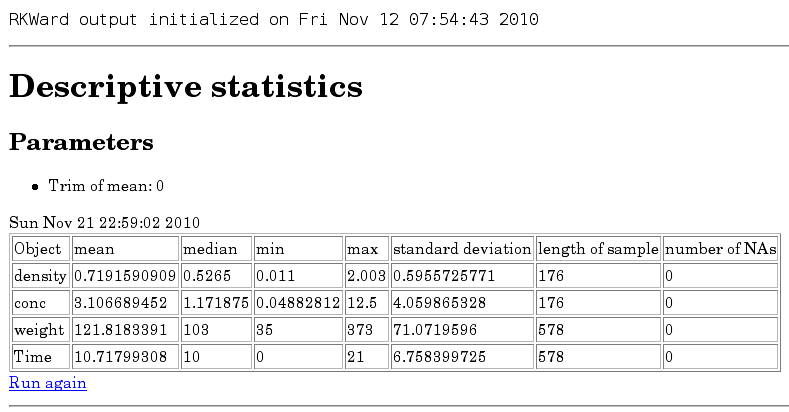
\includegraphics[width=15.5cm]{../figures/results_output_cropped.png}
 \caption{Sample contents of the output window. \code{DNase} data of the \pkg{datasets} package was used. 
  Standard elements of plugin output include a standardized header, and a 
  ``Run again''-link, which allows to repeat the analysis with identical or 
  similar parameters.}
 \label{fig:results_output}
\end{figure}

The formatting of the output is kept to a minimum. In particular,
RKWard is very reluctant to round numerical results for the sake of a
pretty output. Rather, the focus is on making the results easily
accessible for further processing, typically in a dedicated word
processor. Output is based on
\proglang{HTML} (hypertext markup language), and the raw
\proglang{HTML} file and any images therein can be directly
retrieved from a dedicated folder
($\sim\!$/.rkward, by default). It is also
possible to select and copy sections of the output directly from the
output window, and to paste them into office applications as
richly formatted text; even images and tables can be easily copied by drag \& drop to many office applications. In future releases, 
it is planned to integrate RKWard
with existing office suites. This
will possibly also mean addition of different file formats such as ODF (open
document format) and technologies such as \pkg{sweave} and \pkg{odfWeave}
\citep{Leisch2002, Kuhn2006}.

Images contained in the output are stored as
PNG\footnote{\url{http://www.libpng.org/pub/png/}} by
default, but JPEG\footnote{\url{http://www.jpeg.org/index.html}} and
SVG\footnote{\url{http://www.w3.org/Graphics/SVG/}}
can also be used. Similarly, the size of 
images can be configured by the user. It is expected that SVG will
become the default output format eventually, but currently some SVG
files produced by \proglang{R} are not properly
rendered by older supported versions of the
\proglang{KDE} libraries.

\subsection{Package management}
\label{sec:package_management}
The number of \proglang{R} packages available from CRAN (the comprehensive \proglang{R} archive
network), Omegahat\footnote{\url{http://www.omegahat.org/}} and Bioconductor \citep{Gentleman2004} has grown exponentially since \proglang{R}\, 1.3
(2001) to \proglang{R}\, 2.7 (2008) \citep{Fox2008, Ligges2003, Visne2009}. RKWard
utilizes functionality from a growing number of these packages, but avoids
making the installation of all supported packages a pre-requirement to using
RKWard at all. Only once a not yet installed package is required to conduct a certain
action, a package management dialog is invoked automatically, which allows to
download and install the package from a repository such as CRAN. The package
management dialog can also be invoked manually from the menu
(``Settings$\rightarrow$Configure Packages'') for installing new or updating existing \proglang{R}
packages. The underlying package management technology is that of \proglang{R}
\citep{Ligges2003, Ripley2005}.

RKWard supports installing packages to any user writable location. If no current
library location is user writable, RKWard offers to create a new one. 
On UNIX systems, interactively acquiring root privileges for
installation to the system-wide libraries is also supported.
The installation process
itself can be monitored at the interface for error tracking. At the time of this writing, RKWard has no
built-in tools for the interactive exploration of \proglang{R} packages. However, it is
possible to invoke external helpers \citep{Zhang2004}.

\subsection{Further tool windows}
\label{sec:further_tool_windows}

The file browser tool window can be
used to open supported file types (e.\,g., \proglang{R}
scripts, \proglang{HTML} files) inside the main RKWard
window. For unsupported file types (such as PDF; portable document format), the
systems default external applications are used.

The command log window contains a log of the commands that have been
evaluated by the \proglang{R} engine, and any output
produced by these commands. By default, the log shows only commands
which have been entered by the user or directly correspond to user
actions, but it can be configured to include commands which are run for
RKWard's internal purposes such as keeping the workspace browser up
to date.

Commands can be submitted while the \proglang{R} engine
has not yet started, or while another lengthy calculation is still
in progress. In these cases commands are placed into a queue first, and
executed as soon as the \proglang{R} engine becomes
available. The ``pending jobs'' window lists current \proglang{R} commands waiting for
evaluation by the \proglang{R} engine. While this
window is mostly of interest to application developers for diagnostic
purposes, it can also be used to interrupt selected commands.

\subsection{Help system}
\label{sec:help_system}

RKWard provides access to both \proglang{R} specific and 
RKWard specific help pages.
%% TF: Well, I wouldn't really call it seamless. The fact that it's all in one window, and cross-linked is mentioned, below.
% seamlessly in a unified framework. 
\proglang{R} specific documentation includes help pages for functions and packages 
and the various \proglang{R} manuals. RKWard specific documentation consists of
help pages on RKWard in general and on specific GUI dialogs\footnote{For technical 
background of RKWard GUI help pages please refer to Section~\ref{sec:technical_plugins_defining}.}. 
All these various types of help pages can be browsed in the same document 
window, and can be cross--linked. For example, help pages for
RKWard GUI dialogs will typically link to documentation for both
related RKWard dialogs and the underlying \proglang{R} functions.
An arbitrary number of help windows can be browsed simultaneously, in the
TDI view area (see Figure~\ref{fig:main_window}C) or in detached windows.

A central access point to the help system is the ``Help'' menu. Further, help pages on
RKWard GUI dialogs can be accessed from the dialog itself using the
``Help'' button. An useful (``reverse'') feature here is that these pages include 
a link near the top of the page to start the corresponding GUI dialog directly.
Help on \proglang{R} specific functions can be invoked from multiple places, 
such as, the context menu of the workspace browser, by pressing F2 (function
reference) while the cursor is on a function name either in the code editor or 
in the \proglang{R} console, and of course, by using the \proglang{R} \code{help()}
command. In addition, a tool view window is provided as an interface to the
\code{help.search()} command in \proglang{R}. This allows to search all installed, 
all loaded, or specific \proglang{R} packages for a specified topic.

The help browser window is based on the \proglang{KDE}
\proglang{HTML} viewer component and supports many standard
features like increasing or decreasing the font size and searching text
within a page. Additionally, \proglang{R} code inside a help
page can be sent to the \proglang{R} engine for
evaluation by selecting it and pressing F8 (or via ``Run$\rightarrow$Run
Selection'').

% !TEX root = RKWard_paper.tex
\section{Using RKWard -- an example RKWard session}
\label{sec:using_RKWard}
This section describes an example RKWard session, in order to give an idea
of what working with RKWard is like in practice.
The session is organized along the routine tasks of importing,
analyzing, and visualizing data. In this example, it is assumed that an experimental
treatment was given to 20 test subjects. The objective is to compare the responses 
before and after the treatment. 

\subsection{Importing data}
\label{sec:importing_data}
Suppose that the data was saved as or exported to CSV format, for example, from a 
spreadsheet application. RKWard's import plugin can
comfortably read it into a new \proglang{R} object.
The import dialog (``File$\rightarrow$Import$\rightarrow$Import
format$\rightarrow$Import Text/CSV data'') assists in reading the
data by a common point \& click interface (Figure~\ref{fig:import_data}A). In this
example, ``comma'' and ``period'' were chosen via ``Quick mode'' as the field
separator and decimal point characters respectively.

The generated \proglang{R} code can be revealed by clicking on the ``Code'' button:

\code{read.csv(file=`/media/software/experiment.txt', 
na.strings = `NA', nrows = -1, skip = 0,
check.names = TRUE, strip.white = FALSE, blank.lines.skip = TRUE)\\}


Checking the ``Edit Object'' box automatically opens a data editor tab
showing the imported data (Figure~\ref{fig:import_data}B).

\begin{figure}[htp]
 \centering
 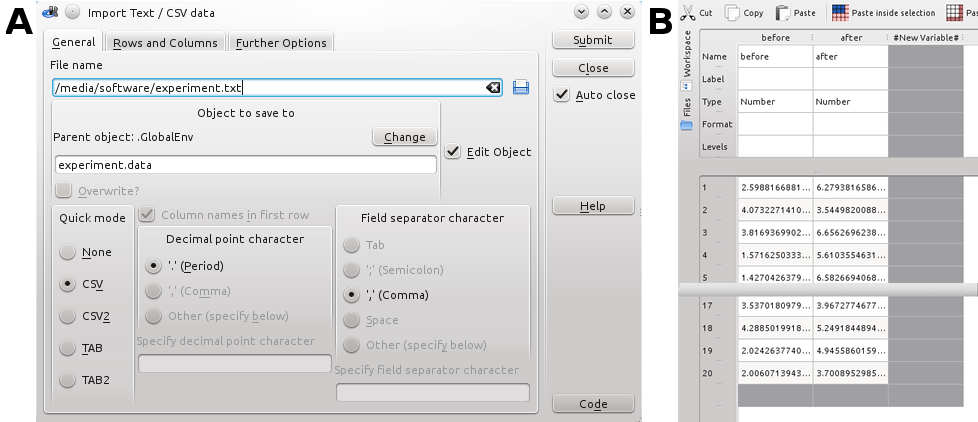
\includegraphics[width=15.5cm]{../figures/import_data.png}
 \caption{A) CSV import dialog. Useful defaults for a variety of common text separated value formats can
  be set using the ``Quick Mode'' selector on the left. Beyond that, many options can be customized. B) Data editor. The imported CSV
  data from experiment.txt are presented (data visually trimmed).}
 \label{fig:import_data}
\end{figure}

\subsection{Conducting a Student's t-test}
\label{sec:conducting_ttest}
To test the hypothesis that the given treatment significantly increased the response, a Student's
t-test for a paired sample is conducted using the 
``Analysis$\rightarrow$Means$\rightarrow$t-Tests$\rightarrow$Two variable t-test'' plugin. 
In the object browser on the left side, the two variables from the expanded
\proglang{R} object containing the table of imported data 
are selected (Figure~\ref{fig:t_test}A). 
Pressing the ``Submit'' button conducts the test, and opens the output document tab
showing the results (Figure~\ref{fig:t_test}B).


\begin{figure}[htp]
 \centering
 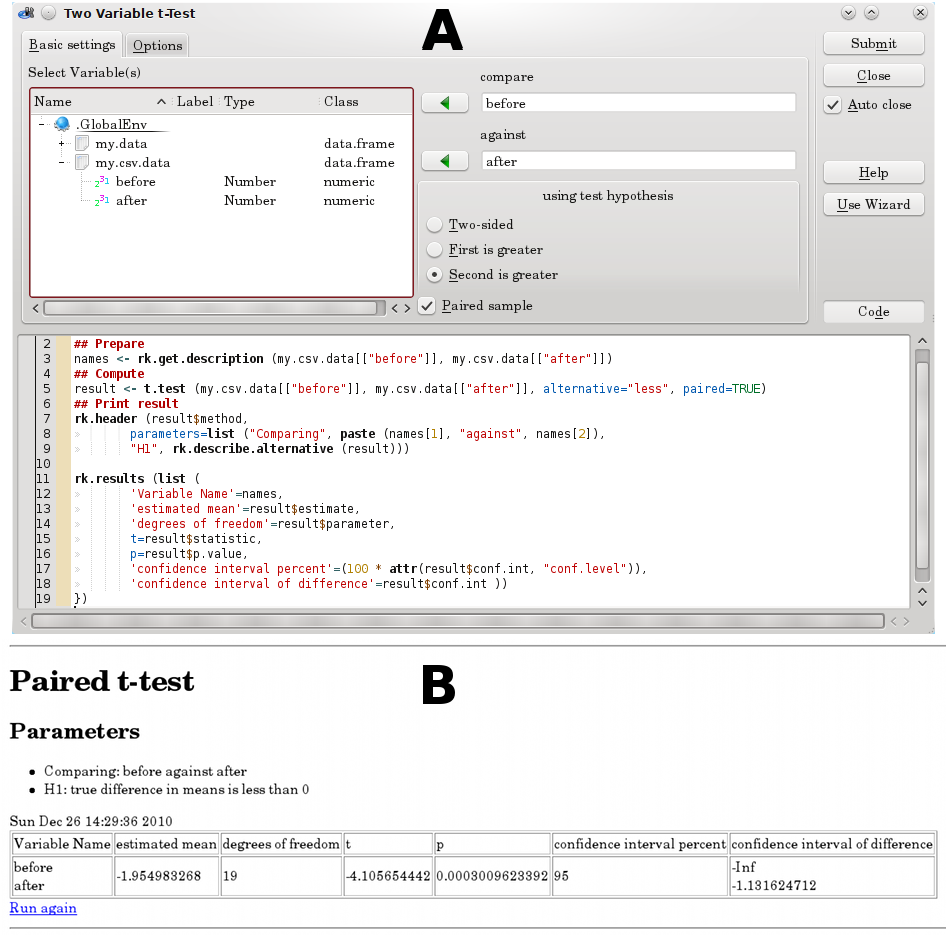
\includegraphics[width=15.5cm]{../figures/t-test2.png}
 \caption{A) Student's t-test dialog for two variables. The bottom area shows the \proglang{R} code corresponding to the settings. 
  B) Test results in tabular \proglang{HTML} format. 
Besides the result, information such as the date of analysis and the relevant test parameters are also reported.}
 \label{fig:t_test}
\end{figure}

\subsection{Creating a plot}
\label{sec:create_plot}
To visualize the data, ``Boxplot'' is chosen from the ``Plots'' menu
and the two variables, corresponding to the t-test above, are selected.
The dialog allows to define custom variable labels (Figure~\ref{fig:boxplot1}).
Checking the ``Preview'' box opens a graphics window showing the boxplot as
it is configured, and updates the window in real time on any changes to plot parameters.
The plot can also be exported to several image formats, directly from the preview window (Figure~\ref{fig:boxplot2}).

\begin{figure}[htp]
 \centering
 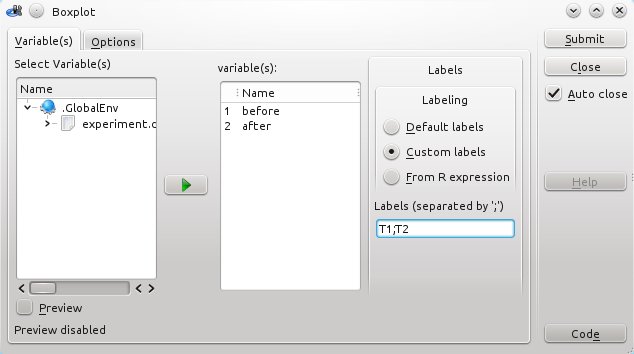
\includegraphics[width=15.5cm]{../figures/boxplot1.png}
 \caption{Boxplot dialog. The first tab ``Variables'' is used to select the variables for analysis. It is possible to
  combine any data present in \code{.GlobalEnv}. The second tab ``Options'' allows further adjustments (e.\,g., the addition of mean and standard deviation) to the plot (not shown).}
 \label{fig:boxplot1}
\end{figure}

\begin{figure}[htp]
 \centering
 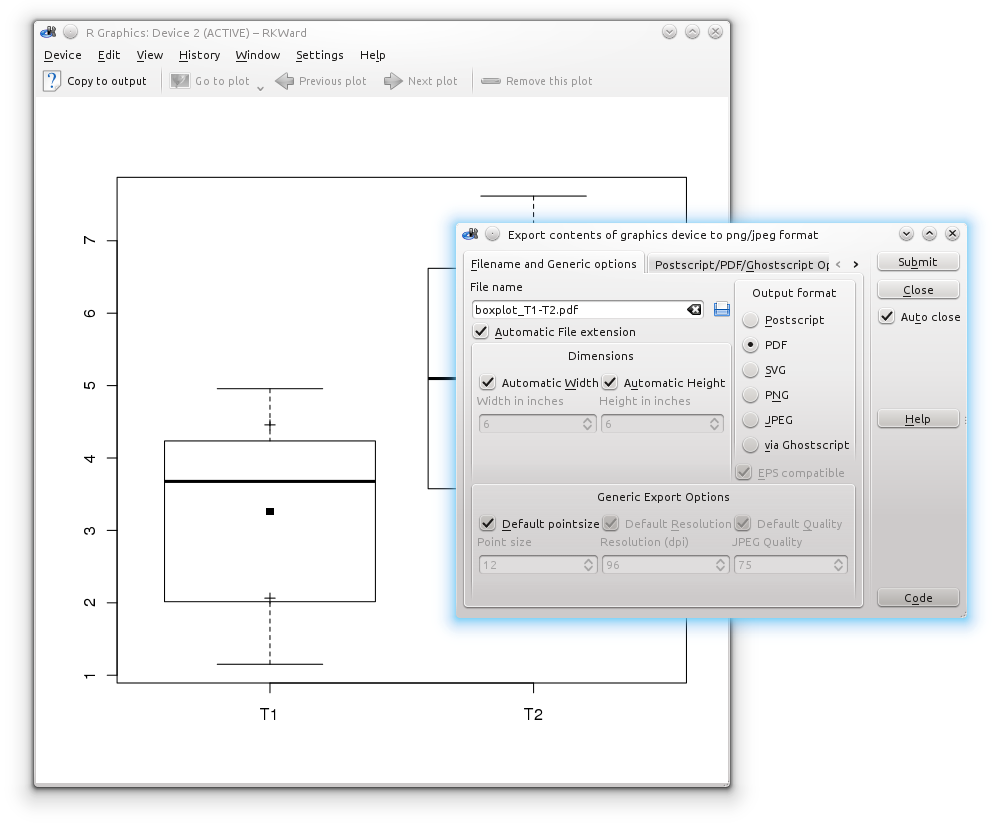
\includegraphics[width=15.5cm]{../figures/boxplot2.png}
 \caption{Plotted data and plot export dialog. The export dialog (``Device$\rightarrow$Export'') provides numerous 
  options like resolution and size for different vector formats (e.\,g., SVG, PDF) and 
  pixel formats (e.\,g., PNG, JPEG). (Note: For the shown figure, the optional  
  mean ($\blacksquare$) and standard deviation ($+$) parameters were selected in the boxplot plugin.)}
 \label{fig:boxplot2}
\end{figure}

%!TEX root=RKWard_paper.tex
\section{Introduction}
In this supplement we will give an overview of some key aspects of \pkg{RKWard}'s
technical design and development process, comparing them briefly to competing GUI solutions, where appropriate.
We will give slightly more attention to the details of the
plugin framework (Section~\ref{sec:technical_plugins}) used in \pkg{RKWard}, since this is central to the extensibility of
\pkg{RKWard}, and we will conclude with an example for extending \pkg{RKWard} by a plugin (Section~\ref{sec:example_plugin}).

\section{Asynchronous command execution}
\label{sec:technical_asynchronous}
One central design decision in the implementation of \pkg{RKWard} is that the
interface to the \proglang{R} engine operates asynchronously. The intention is to
keep the application usable to a high degree, even during the computation of
time-consuming analysis. For instance, while waiting for the estimation of a
complex model to complete, the user should be able to continue to use the GUI to
prepare the next analysis. Asynchronous command execution is also a prerequisite
for an implementation of the plot-preview feature (see the section no graphics windows
in the main article). Internally, the GUI frontend and the \proglang{R} engine run in two separate processes\footnote{
    Up to \pkg{RKWard} version 0.5.4, two separate threads inside a single process were used. This alternate design is still
    available as a compile time option.
}. Commands generated from plugins or user actions are placed in queue in the frontend and are evaluated in
the backend process in the order they were submitted\footnote{
    It is possible, and in some cases necessary, to enforce a different order of command execution in
    internal code. For instance, \pkg{RKWard} makes sure that no user command can
    potentially interfere while \pkg{RKWard} is loading the data of a \code{data.frame} for
    editing.
}.

The asynchronous design implies that \pkg{RKWard} avoids relying on the
\proglang{R} engine during interactive use. This is one of several reasons for
the use of \proglang{ECMAScript} in plugins, instead of scripting using
\proglang{R} itself (see Sections~\ref{sec:technical_toolkit} and \ref{sec:technical_plugins}).
A further implication is that \pkg{RKWard} avoids querying information about the
existence and properties of objects in \proglang{R} interactively. Rather,
\pkg{RKWard} keeps a representation of \proglang{R} objects and their basic properties
(e.\,g., class and dimensions), which is used for the workspace browser,
object name completion, function argument hinting, and
other places. The object representation includes objects in all environments
in the search path, and any objects contained within these environments in a
hierarchical tree\footnote{
    Currently, environments of functions or formulas are not taken into account, but slots of S4 objects,
    and package namespace environments are represented in the object tree.
}. The representation of \proglang{R} objects is gathered
pro-actively\footnote{
    To limit the amount of processing, and to avoid recursion, \pkg{RKWard} currently stops
    gathering object information at a depth of three levels. Information on deeper levels is gathered
    on an as-needed basis, when the user accesses information on the respective parent objects.
}. This has a notable impact on performance when loading packages.
Specifically, objects which would usually be ``lazy loaded'' only when needed \citep[see][]{Ripley2004} are
accessed in order to fetch information on their properties. This means the data
has to be loaded from disk; however, the memory is freed immediately after fetching
information on the object. Additionally, for packages with extremely large number of objects, \pkg{RKWard}
provides an option to exclude specific packages from scanning the object structures.

A further side-effect of the asynchronous threaded design is that there is
inherently a rather clear separation between the GUI code and the code making direct use
of the \proglang{R} application programming interface (API) (see also Figure~\ref{fig:design_sketch}). 
In future releases it could be made possible to run GUI and \proglang{R} engine on different computers.

\begin{figure}[t!]
 \centering
 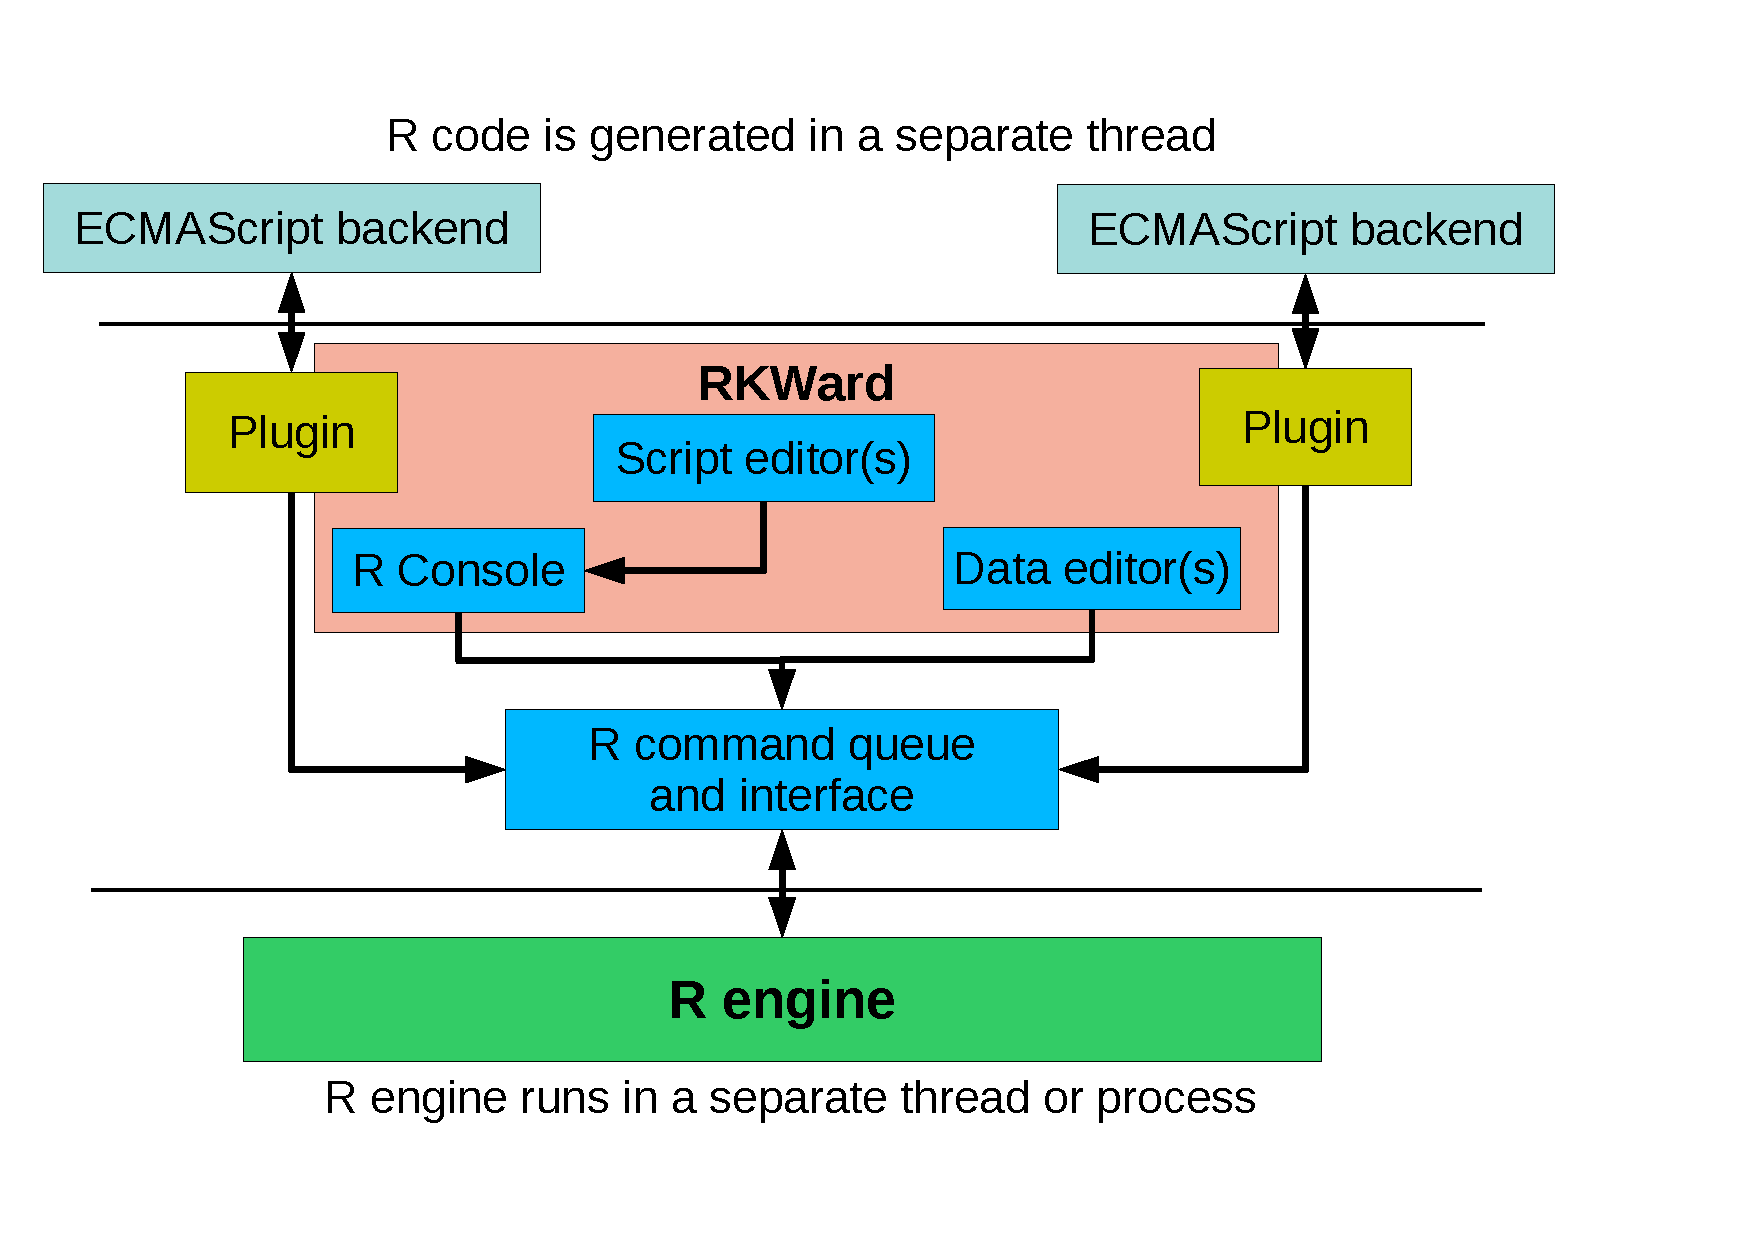
\includegraphics[clip=true,trim=0cm 2cm 0cm 0cm]{./figures/design_sketch.pdf}
 \caption{Technical design of \pkg{RKWard}. Only a few central components are visualized.
 All communication with the \proglang{R} engine is passed through a single interface living in the frontend process. The \proglang{R} engine itself
 runs in a separate process. 
 Separate threads within the frontend process are used to generate \proglang{R} code from plugins.
}
 \label{fig:design_sketch}
\end{figure}

\section{Object modification detection}
\label{sec:technical_omd}
\pkg{RKWard} allows the user to run arbitrary commands in \proglang{R} at any time, even while
editing a \code{data.frame} or while selecting objects for analysis in a GUI dialog. Any user
command can potentially add, modify, or remove objects in \proglang{R}. \pkg{RKWard} tries to
detect such changes in order to always display accurate information in the
workspace browser, object selection lists, and object views. Beyond that,
detecting any changes is particularly important with respect to objects which
are currently being edited in the data editor (which provides an illusion
of in-place editing, see the section on the spreadsheet-like data editor in the
main article). Here, it is necessary to synchronize
the data between \proglang{R} and the GUI in both directions.

For simplicity and performance, object modification detection is only
implemented for objects inside the ``global environment'' (including environments
inside the global environment), since this is where changes are typically done.
Currently, object modification detection is based on active bindings.
Essentially, any object which is created in the global environment is first
moved to a hidden storage environment, and then replaced with an active binding.
The active binding acts as a transparent proxy to the object in the storage
environment, which registers any write-access to the object\footnote{
    This is similar to the approach taken in the \pkg{trackObjs} package \citep{Plate2009}.
}.

The use of active bindings has significant performance implications when
objects are accessed very frequently. This is particularly notable where an
object inside the global environment is used as the index variable in a loop,
as illustrated by the following example. When control returns to the top level
prompt, after the first assignment, \code{i} will become subject to object modification
detection (i.\,e., it will be wrapped into an active
binding). The subsequent \code{for} loop will then run slow.

\begin{Code}
R> i <- 1
R> for (i in 1:100000) i + i
\end{Code}

In contrast, in the following example, \code{i} is a local object, and will not
be replaced by an active binding. Therefore the loop will run approximately as fast
as in a plain \proglang{R} session:

\begin{Code}
R> f <- function () {
R+    i <- 1
R+    for (i in 1:100000) i + i
R+ }
R> f ()
\end{Code}

Future versions of \pkg{RKWard} will try to avoid this performance problem. 
One approach that is currently under consideration is to simply perform
a pointer comparison of the \code{SEXP} records of objects in global environment with
their copies in a hidden storage environment. Due to the implicit sharing of
\code{SEXP} records \citep{RDCT2010a, RDCT2010b}, this should provide for a reliable
way to detect changes for most types of \proglang{R} objects, with comparatively low memory
and performance overhead. Special handling will be needed for environments and
active bindings.

\section{Choice of toolkit and implementation languages}
\label{sec:technical_toolkit}
In addition to \proglang{R}, \pkg{RKWard} is based on the \pkg{KDE} libraries, which are in turn based
on \pkg{Qt}, and implemented mostly in \proglang{C++}. Compared to many competing libraries,
this constitutes a rather heavy dependency. Moreover, the \pkg{KDE} libraries are
still known to have portability issues especially on Mac OS X, and to some degree
also on the Microsoft Windows platform \citep{Jarvis2010}.

The major reason for choosing the \pkg{KDE} and \pkg{Qt} libraries has been the 
many high level features, they provide. This has allowed \pkg{RKWard} development to make quick
progress despite limited resources. Most importantly, the \pkg{KDE} libraries provide a
full featured text editor \citep{CullmannND} as a component which can be
seamlessly integrated into a host application using the KParts technology
\citep{Faure2000}. Additionally, another KPart provides HTML browsing capabilities in a
similarly integrated way. The availability of \pkg{KWord} \citep{KWord} as an
embeddable KPart might prove useful in future versions of \pkg{RKWard}, when better
integration with office suites will be sought.

Another technology from the \pkg{KDE} libraries that is important to the development
of \pkg{RKWard} is the ``XMLGUI'' technology
\citep{Faure2000}. This is especially helpful in providing an integrated GUI across
the many different kinds of document windows and tool views supported in \pkg{RKWard}.

Plugins in \pkg{RKWard} rely on XML\footnote{\url{http://www.w3.org/XML/}}
and \proglang{ECMAScript}\footnote{\url{http://www.ecmascript.org/}} (see Section~\ref{sec:technical_plugins}). XML is not
only well suited to describe the layout of the GUI of plugins, but simple
functional logic can also be represented \citep[see also][]{Visne2009}. \proglang{ECMAScript} was
chosen for the generation of \proglang{R} commands within plugins, in particular due to its
availability as an embedded scripting engine inside the \pkg{Qt} libraries. While at
first glance \proglang{R} itself would appear as a natural choice of scripting language as
well, this would make it impossible to use plugins in an asynchronous way.
Further, the main functional requirement in this place is the manipulation and
concatenation of text strings. While \proglang{R} provides support for this, concatenating
strings with the \code{+}-operator, as available in \proglang{ECMAScript}, allows for a
very readable way to perform such basic text manipulation.

\section{On-screen graphics windows}
\label{sec:technical_graphics}
Contrary to the approach used in \pkg{JGR} \citep{JGR2010}, \pkg{RKWard} does
not technically provide a custom on-screen graphics device. \pkg{RKWard} detects when
new graphics windows are created via calls to \code{X11()} or \code{windows()}. These windows
are then ``captured'' in a platform dependent way (based on the XEmbed \citep{Ettrich2002} protocol
for \pkg{X11}, or on reparenting for the Microsoft Windows platform). An \pkg{RKWard} menu bar and a
toolbar is then added to these windows to provide added functionality. While
this approach requires some platform dependent code, any corrections or
improvements made to the underlying \proglang{R} native devices will automatically be
available in \pkg{RKWard}.

A recent addition to the on-screen device is the ``plot history'' feature which
adds a browsable list of plots to the device window. Since \pkg{RKWard} does not use a
custom on-screen graphics device, this feature is implemented in a package
dependent way. For example, as of this writing, plotting calls that use either
the ``standard graphics system'' or the ``\pkg{lattice} system'' can be added to the plot
history; other plots are drawn but not added. The basic procedure is to identify
changes to the on-screen canvas and record the existing plot before a new plot
wipes it out. A single global history for the recorded plots is maintained
which is used by all the on-screen device windows. This is similar to the
implementation in \proglang{Rgui.exe} (Microsoft Windows), but unlike the one in \proglang{Rgui.app} 
(Mac OS X). Each such device window points to a position in the history
and behaves independently when recording a new plot or deleting an existing
one.

Plot history support for the
\pkg{lattice} system \citep{Sarkar2008} is implemented by inserting a hook in the \code{print.lattice()}
function. This hook retrieves and stores the \code{lattice.status} object from the
\code{lattice:::.LatticeEnv} environment, thereby making \code{update()} calls on trellis
objects transparent to the user. Any recorded trellis object is then replayed
using \code{plot.lattice()}, bypassing the recording mechanism. The standard graphics
system, on the other hand, is implemented differently because the hook in
\code{plot.new()} is ineffective for this purpose. A customized function is overloaded
on \code{plot.new()} which stores and retrieves the existing plot, essentially, using
\code{recordPlot()} and replays them using \code{replayPlot()}.

The actual plotting calls are tracked using appropriate \code{sys.call()} commands in
the hooks. These call strings are displayed as a drop-down menu on the toolbar
for non-sequential browsing (see the section on graphics windows in the main article) providing a very intuitive browsing
interface unlike the native implementations in \code{windows()} and \code{quartz()} devices.

\section{Plugin infrastructure}
\label{sec:technical_plugins}
One of the earliest features of \pkg{RKWard} was the extensibility by plugins.
Basically, plugins in \pkg{RKWard} provide complete GUI dialogs, or re-usable
GUI components, which accept user settings and translate those user settings
into \proglang{R} code\footnote{
    Plugins are also used in some other contexts within \pkg{RKWard}, for instance, the
    integrated text editor (\pkg{kate} part) supports extensions via plugins and user scripts. At this point we
    will focus only on plugins generating \proglang{R} code.
}. Thus, the plugin framework is basically a tool set used to define
GUIs for the automatic generation of \proglang{R} code.

Much of the functionality in \pkg{RKWard} is currently implemented as plugins. For example, importing different file
formats relying on the \pkg{foreign} package is achieved by this approach. Similarly,
\pkg{RKWard} provides a modest GUI driven tool set for statistical analysis,
especially for item response theory, distributions, and descriptive
statistical analysis.

\subsection{Defining a plugin}
\label{sec:technical_plugins_defining}
Plugins consist of four parts as visualized in Figure~\ref{fig:plugin_structure} 
\citep[see Section~\ref{sec:example_plugin} for an example; for a complete
manual, see][]{Friedrichsmeier2010}:

\begin{figure}[t!]
 \centering
 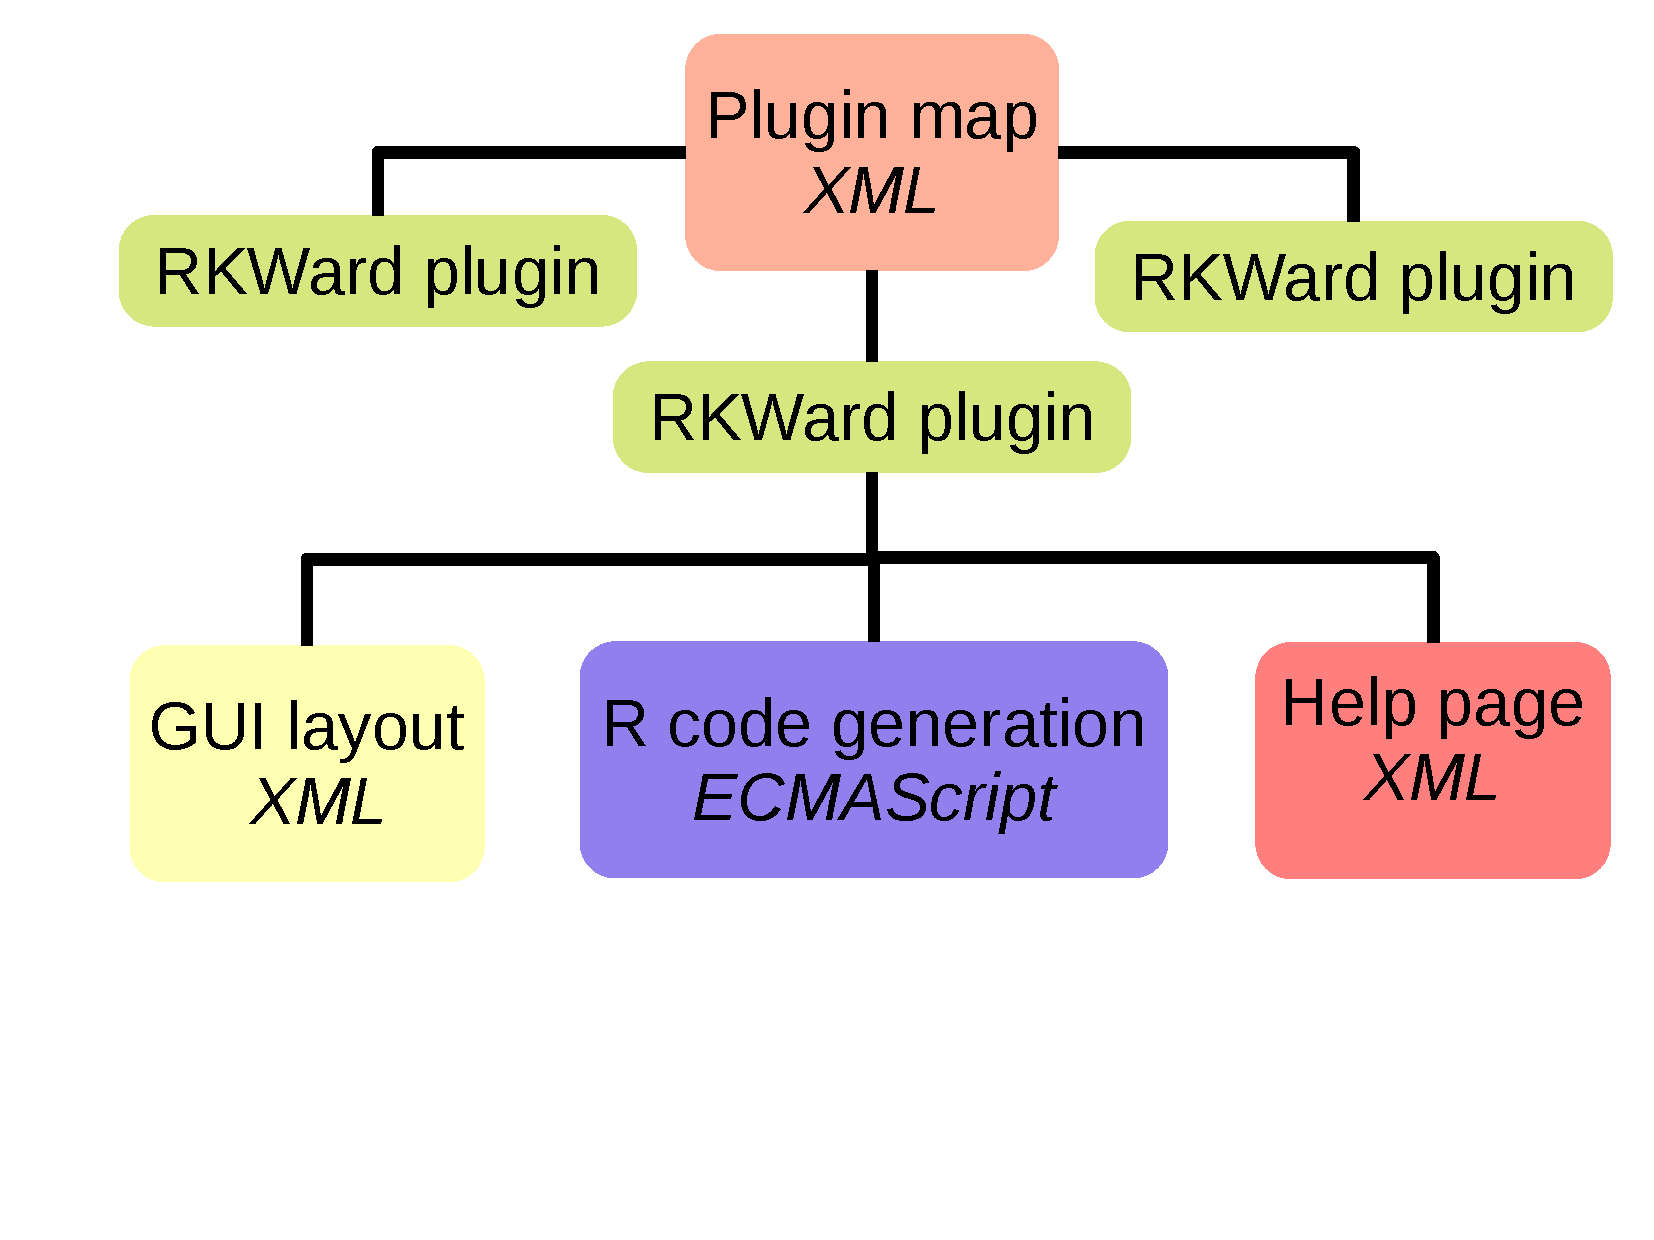
\includegraphics[clip=true,trim=0cm 6cm 0cm 0cm,width=8cm]{./figures/plugin_structure.pdf}
 \caption{Plugin structure of \pkg{RKWard}. One or more plugins are declared in a ``plugin map''. Each plugin is defined by
 two XML files, and one \proglang{ECMAScript} file.}
 \label{fig:plugin_structure}
\end{figure}

\begin{itemize}
    \item
    An XML file (Section~\ref{sec:defining_menu_hierarchy}), 
    called a ``plugin map'', is used to declare one or more plugins, each
    with a unique identifier. For most plugins, the plugin map also defines the
    placement in the menu hierarchy. Plugin maps are meant to represent groups of
    plugins. Users can disable/enable such groups of plugins in order to reduce the
    complexity of the menu hierarchy.

    \item
    A second XML file describes the plugin GUI layout itself (Section~\ref{sec:defining_dialog_ui}). 
    Most importantly this includes
    the definition of the GUI layout and GUI behavior. High level GUI elements can
    be defined with simple XML-tags. Layout is based on ``rows'' and ``columns'',
    instead of pixel counts. In most cases this allows for a very sensible resizing
    behavior. \pkg{RKWard} supports single-page dialogs and multi-page wizards, however,
    most plugins define only a single-page GUI. GUI behavior can be programmed by
    connecting ``properties'' of the GUI elements to each other. For example, the state
    of a checkbox could be connected to the ``enabled'' property of a dependent
    control. More complex logic is also supported, as is procedural scripting of GUI
    behavior using \proglang{ECMAScript}.

    \item
    A separate \proglang{ECMAScript} file (Section~\ref{sec:generating_r_code_from_ui_settings}) 
    is used to translate GUI settings into \proglang{R}
    code\footnote{
        In earlier versions of \pkg{RKWard}, \proglang{PHP} was used
        as a scripting engine, and \proglang{PHP} interpreters were run as separate processes.
        Usage of \proglang{PHP} was abandoned in \pkg{RKWard} version 0.5.3 for reasons of performance and simplicity.
    }. This \proglang{ECMAScript} file is evaluated asynchronously in a separate thread. \pkg{RKWard}
    currently enforces structuring the code into three separate sections for
    preprocessing, calculating, and printing results. The generated code is always
    run in a local environment, in order to allow the use of temporary variables
    without the danger of overwriting user data.

    \item
    A third XML file defines a help page. This help page usually links to the \proglang{R} help
    pages of the main functions/concepts used by the plugin, as well as to other
    related \pkg{RKWard} help pages. Compared to \proglang{R} help
    pages, the plugin help pages try to give more hands-on advice on using the
    plugin. Plugins can be invoked from their help page by clicking on a link near
    the top, which can be useful after following a link from a related help page.
\end{itemize}

Changes to the source code of these elements take effect without the requirement to recompile \pkg{RKWard}.

\subsection{Embedding and reuse of plugins}
\label{sec:technical_plugins_embedding}
\pkg{RKWard} supports several mechanisms for modularization and re-use of
functionality in plugins. File inclusion is one very simple but effective
mechanism, which can be used in the \proglang{ECMAScript} files, but is also supported in
the XML files. In script files, this is most useful by defining common functions
in an included file. For the XML files, the equivalent is to define ``snippets''
in the included file, which can then be inserted.

A third mechanism allows to completely embed one plugin into another. For
instance the \code{plot\_options} plugin is used by many plugins in \pkg{RKWard}, to provide
common plot options such as labels, axis options, and grids. Other plugins
can embed it using the \code{embed}-tag in their XML file (the plugin supports
hiding irrelevant options). The generated code portions can be fetched from the
\proglang{ECMAScript} file just like any other GUI settings, and inserted into the complete
code. Other examples of embedded plugins are options for histograms, barplots,
and empirical cumulative distribution function (ECDF) plots (which in turn embed the generic plot options plugin).

\subsection{Enforcing a consistent interface}
\label{sec:technical_plugins_consistency}
\pkg{RKWard} tries to make it easy to create a consistent interface in all plugins.
GUI-wise this is supported by providing high-level GUI elements, and embeddable
clients. Also, the standard elements of each dialog (``Submit'', and
``Cancel'' buttons, on-the-fly code view, etc.) are hard coded. Up to version
0.5.3 of \pkg{RKWard} it was not possible to use any GUI elements in plugins which
were not explicitly defined for this purpose. In the current development
version, theoretically, all GUI elements available from \pkg{Qt} can be inserted,
where necessary.

For generating output, the function \code{rk.header()} can be used to print a
standardized caption for each piece of output. Printing results in vector or
tabular form is facilitated by \code{rk.results()}. A wide range of objects can be
printed using \code{rk.print()}, which is just a thin wrapper around the
\code{HTML()} function of the \pkg{R2HTML} package \citep{Lecoutre2003} in the current
implementation. The use of custom formatting with HTML is possible, but
discouraged. Standard elements such as a horizontal separator, and the ``Run again''
link (see the section on the results output in the main article) are inserted automatically, without the need to define
them for each plugin.

Regarding the style of the generated \proglang{R} code, enforcing consistency is harder,
but plugins which are to become part of the official \pkg{RKWard} application are
reviewed for adherence to some guidelines. Perhaps the most important guidelines
are 

\begin{itemize}
  \item 
  Write readable code, which is properly indented, and commented where necessary.

  \item 
  Do not hide any relevant computations from the user by performing them in the
  \nobreak{\proglang{ECMAScript}}. Rather, generate \proglang{R} code which will perform
  those computations, transparently.

  \item
  Plugins can be restricted to accept only certain types of data (such as only one-dimensional numeric data).
  Use such restrictions where appropriate to avoid errors, but be very careful not to add
  too many of them.
\end{itemize}

\subsection[Handling of R package dependencies]{Handling of \proglang{R} package dependencies}
\label{sec:technical_plugins_dependencies}
A wide range of plugins for diverse functionality is present in \pkg{RKWard},
including plots (e.\,g., boxplot) or standard tests (e.\,g., Student's t-test)\footnote{
  At the time of this writing, there are 164 user-accessible plugins in \pkg{RKWard}.
  Listing all is beyond the scope of this article.
}. Some
of the plugins depend on \proglang{R} packages other than the recommended \proglang{R} base packages.
Examples herein are the calculation of kurtosis, skewness or the exact Wilcoxon
test.

\pkg{RKWard} avoids loading all these packages pro-actively, as \pkg{Rcmdr} does. Rather,
plugins which depend on a certain package simply include an appropriate call to
\code{require()} in the pre-processing section of the generated \proglang{R} code. The \code{require()}
function is overloaded in \pkg{RKWard}, in order to bring up the package-installation
dialog whenever needed. Packages invoked by \code{require()} remain loaded
in the active \pkg{RKWard} session unless unloaded manually (from the workspace browser, or using the
\proglang{R} function \code{detach()}).

Dependencies between (embedded) plugins are handled using the \code{<require>}-tag in the plugin map.

\subsection{Development process}
\subsubsection[RKWard core and external plugins]{\pkg{RKWard} core and external plugins}
\label{sec:technical_processes_plugins}
Newly developed plugins are placed in a dedicated plugin map file.
Plugins in this map are not visible to the user by
default, but need to be enabled manually. Once the author(s) of a plugin
announces that they consider it stable, the plugin is subjected to a review for
correctness, style, and usability. The review status is tracked in the project
wiki. Currently at least one positive review is needed before the plugin is
allowed to be made visible by default, by moving it to an appropriate plugin
map.

The current development version adds support for downloading additional sets of
plugins, which are neither officially included nor supported by the
\pkg{RKWard} developers, from the internet.

\subsubsection{Automated testing}
\label{sec:technical_processes_automatedtesting}
A second requirement for new plugins is that each plugin must be accompanied by
at least one automated test. The automated testing framework in \pkg{RKWard} consists
of a set of \proglang{R} scripts which allow to run a plugin with specific GUI settings,
automatically\footnote{
  In the current development version, the scripts have been converted into a proper
  \proglang{R} package.
}. The resulting \proglang{R} code, \proglang{R} messages, and output are then compared
to a defined standard. Automated tests are run routinely after changes in the
plugin infrastructure, and before any new release.

The automated testing framework is also useful in testing some aspects of the
application which are not implemented as plugins, but this is currently limited
to very few basic tests.

% !TEX root = RKWard_paper.tex
\section{Extending RKWard - an example of creating a plugin}
\label{sec:example_plugin}
As discussed in Section~\ref{sec:technical_plugins}, plugins in RKWard are
defined by four separate files (Figure~\ref{fig:plugin_structure}). To give an impression of the technique,
this section shows (portions of) the relevant files for a plugin that provides
a simple dialog for a t-test. For brevity, the help-file is omitted.

\subsection{Defining the menu hierarchy}
\label{sec:defining_menu_hierarchy}
A so called ``.pluginmap'' file declares each plugin, and, if appropriate, defines where it should
be placed in the menu hierarchy. Usually each .pluginmap-file declares many plugins. In this example
we only show one, namely,
%% TF: Well, I don't think this is really a feature to advertize. We don't actually support this,
%% and any changes would be overwritten by the next update.
%Since the files are editable with a text editor it is possible for the user to adjust
%the menus as desired.
the definition entry for a two variable t-test (see Figure~\ref{fig:ttest-gui-example}). 
The pluginmap (\code{<!DOCTYPE rkpluginmap>}) gives a unique identifier (``id"), the location of the GUI description (``file"), and the window title (``label''). The menu
is defined in a hierarchical structure (see code example below; long lines are broken at ``$\ldots~\ldots$''). Moreover, the position within the menu can be explicitly defined.
This might be required if the menu entries are to be ordered non-alphabetically.

\begin{footnotesize}
\begin{Code}
<!DOCTYPE rkpluginmap>

<document base_prefix="" namespace="rkward">
  <components>
    <component type="standard" id="t_test_two_vars" file="analysis/t_test_two_vars.xml" ...
      ... label="Two Variable t-test" />
  </components>

  <hierarchy>
    <!-- Menu hierarchy can be defined in XML, easily.
    Menus with the same "id"-attribute will be merged, even if defined in
    separate .pluginmap files. -->
    <menu id="analysis" label="Analysis" index="4">
      <menu id="means" label="Means" index="4">
        <menu id="ttests" label="t-Tests">
          <entry component="t_test_two_vars" />
        </menu>
      </menu>
    </menu>
  </hierarchy>
</document>
\end{Code}
\end{footnotesize}

\begin{figure}[htp]
 \centering
 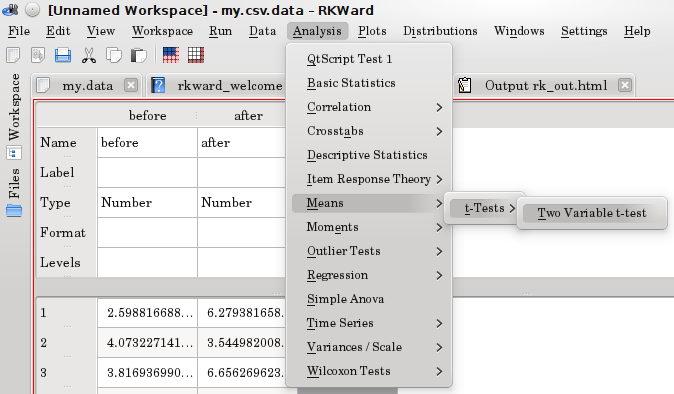
\includegraphics{../figures/ttest-gui-example.png}
 \caption{Generated menu GUI as defined by the pluginmap.}
 \label{fig:ttest-gui-example}
\end{figure}


\subsection {Defining the dialog UI}
\label{sec:defining_dialog_ui}
The main \proglang{XML} file of each plugin defines the layout and behavior of the GUI, and references the
\proglang{ECMAScript} file that is used for generating \proglang{R} code from UI settings and the help file (not included in this paper).

Some GUI behavior can also be scripted in \proglang{ECMAScript}. In this example, the logic is defined in \proglang{XML} (the ``Assume equal variances'' checkbox
is only enabled for paired sample tests).

The \proglang{XML} file defines the t-test plugin (\code{<!DOCTYPE rkplugin>}) to be organized in two tabs (Figure~\ref{fig:t_test}A) asking for the variables
to analyze in the first tab and optionally in the second tab for specific settings like the confidence level (default 0.95). Note that this \proglang{XML} file
also invokes the \proglang{XML} help file. Two variables can be selected (\code{<varslot .../>}). These are set to be ``required'', i.e.
the ``Submit'' button will remain disabled until the user has made a valid selection for both.


\begin{footnotesize}
\begin{Code}
<!DOCTYPE rkplugin>
<document>
  <code file="t_test_two_vars.js"/>
  <help file="t_test_two_vars.rkh"/>

  <logic>
    <!-- GUI behavior can also be scripted in ECMAScript. -->
    <connect client="varequal.enabled" governor="paired.not"/>
  </logic>

  <dialog label="Two Variable t-Test">
    <tabbook>
      <tab label="Basic settings" id="tab_variables">
        <row id="basic_settings_row">
          <varselector id="vars"/>
          <column>
            <varslot type="numeric" id="x" source="vars" required="true"
              label="compare"/>                                                             
            <varslot type="numeric" id="y" source="vars" required="true"
              label="against"/>
            <radio id="hypothesis" label="using test hypothesis">
              <option value="two.sided" label="Two-sided"/>
              <option value="greater" label="First is greater"/>
              <option value="less" label="Second is greater"/>
            </radio>
            <checkbox id="paired" label="Paired sample" value="1" value_unchecked="0" />
          </column>
        </row>
      </tab>
      <tab label="Options" id="tab_options">
        <checkbox id="varequal" label="assume equal variances" value="1"
          value_unchecked="0"/>
        <frame label="Confidence Interval" id="confint_frame">
          <spinbox type="real" id="conflevel" label="confidence level" min="0" max="1"
            initial="0.95"/>
          <checkbox id="confint" label="print confidence interval" value="1"
            checked="true"/>
        </frame>
        <stretch/>
      </tab>
    </tabbook>
  </dialog>
</document>
\end{Code}
\end{footnotesize}

\subsection{Generating R code from UI settings}
\label{sec:generating_r_code_from_ui_settings}
A simple \proglang{ECMAScript} script is used to generate \proglang{R} code from UI settings (using \code{echo()} commands).
Generated code for each plugin is divded into three sections: ``Preprocess'', ``Calculate'', and ``Printout'', although each
may be empty.

\begin{footnotesize}
\begin{Code}
// globals
var x;
var y;
var varequal;
var paired;

function preprocess () {
  x = getValue ("x");
  y = getValue ("y");

  echo ('names <- rk.get.description (' + x + ", " + y + ')\n');
}

function calculate () {
  varequal = getValue ("varequal");
  paired = getValue ("paired");

  var conflevel = getValue ("conflevel");
  var hypothesis = getValue ("hypothesis");

  var options = ", alternative=\"" + hypothesis + "\"";
  if (paired) options += ", paired=TRUE";
  if ((!paired) && varequal) options += ", var.equal=TRUE";
  if (conflevel != "0.95") options += ", conf.level=" + conflevel;

  echo ('result <- t.test (' + x + ", " + y + options + ')\n');
}

function printout () {
  echo ('rk.header (result\$method, \n');
  echo ('  parameters=list ("Comparing", paste (names[1], "against", names[2]),\n');
  echo ('  "H1", rk.describe.alternative (result)');
  if (!paired) {
    echo (',\n');
    echo ('  "Equal variances", "');
    if (!varequal) echo ("not");
    echo (' assumed"');
  }
  echo ('))\n');
  echo ('\n');
  echo ('rk.results (list (\n');
  echo ('  \'Variable Name\'=names,\n');
  echo ('  \'estimated mean\'=result\$estimate,\n');
  echo ('  \'degrees of freedom\'=result\$parameter,\n');
  echo ('  t=result\$statistic,\n');
  echo ('  p=result\$p.value');
  if (getValue ("confint")) {
    echo (',\n');
    echo ('  \'confidence interval percent\'=(100 * attr(result\$conf.int, "conf.level")),\n');
    echo ('  \'confidence interval of difference\'=result\$conf.int ');
  }
  echo ('))\n');
}
\end{Code}
\end{footnotesize}

The generated code readable by the user is the following \proglang{R} code. Here, \code{rk.header} and \code{rk.results} 
are RKWard functions provided by the package \pkg{rkward}. In case the package is installed the code below 
can be run from any \proglang{R} engine.

\begin{footnotesize}
\begin{Code}
local({
## Prepare
names <- rk.get.description (my.csv.data[["before"]], my.csv.data[["after"]])
## Compute
result <- t.test (my.csv.data[["before"]], my.csv.data[["after"]], alternative="less", paired=TRUE)
## Print result
rk.header (result$method, 
	parameters=list ("Comparing", paste (names[1], "against", names[2]),
	"H1", rk.describe.alternative (result)))

rk.results (list (
	'Variable Name'=names,
	'estimated mean'=result$estimate,
	'degrees of freedom'=result$parameter,
	t=result$statistic,
	p=result$p.value,
	'confidence interval percent'=(100 * attr(result$conf.int, "conf.level")),
	'confidence interval of difference'=result$conf.int ))
})

\end{Code}
\end{footnotesize}

\section{Conclusion and outlook}
\label{sec:conclusion_summary}
In this article we have introduced the RKWard GUI to \proglang{R}. RKWard provides features ranging
from easy to use dialogs for common statistical procedures, targetted at \proglang{R} novices, to advanced
IDE features targetted at \proglang{R} experts.

RKWard tries to empower users of all knowledge levels to make more efficient use of the 
\proglang{R} programming language, while carefully avoiding to lock in users to a specific
GUI solution. In particular, RKWard
\begin{itemize}
 \item provides full transparency about the \proglang{R} code that is used to carry out tasks.
 \item avoids introducing RKWard-specific \proglang{R} functions for central functionality (but uses some for output formatting).
 \item avoids hard dependencies on third-party \proglang{R} packages.
 \item uses standard \proglang{R} formats \citep[cf.][]{RDCT2010c} for data storage, and open standards (\proglang{HTML}, \proglang{PNG}, \proglang{SVG}) for storage of output.
\end{itemize}

%% TF: I don't think this comparison is entirely fair. Keep in mind that this is is a special issue about R GUIs.
%% So all those GUIs will base their calculations on R. But some will do it more transparently than others.
%The RKWard development 
%does not focus on \proglang{R} package development, except those internally 
%required for RKWard, but keeps it at the \proglang{R} community. This design brings the intrinsic 
%benefit of highly accurate results since calculations entirely rely on \proglang{R} code. 
%Comparison of the commonly used spreadsheet applications 
%regarding estimation, random number generation and statistical distributions revealed serious 
%limitations. \proglang{R} in contrast was found to be a reliable and accurate statistical 
%software package \citep{Almiron2009, Almiron2010}.

\proglang{R} scripts which are routinely in use or require complex steps can be programmed as GUI 
elements in RKWard. Due to its plugin architecture RKWard provides the basis 
for a highly customizable \proglang{R}-GUI. We show that the plugin development can take place 
independently without changes in the core application or compilation of binaries. 
Current developments also targets plugin development via external canals like 
GHNS (Get Hot New Stuff)\footnote{\url{http://ghns.freedesktop.org/}} independently of the 
RKWard plugin development. 
Future versions of RKWard will continue to add value for both groups of users. Planned features include
an enhanced interface for debugging \proglang{R} code, support for editing more types of data, and the
ability to connect the RKWard GUI to a remote \proglang{R} engine. Perhaps most importantly, RKWard will
gain many new UI dialogs for manipulation, analysis, and visualization of data. The ability to
develop these dialogs as plugins allows any contributor or user to help in enhancing RKWard, without in-depth
programming knowledge.

\section{Acknowledgments}
\label{sec:acknowledgments}
The work described in this paper was supported by YOUR NAME OR THE NAME
OF SOMEBODELSE HERE


\bibliography{sources}
\end{document}
